\documentclass[11pt,titlepage,headings,oneside,openany]{book}
\usepackage{kotex}
\usepackage{graphicx}
\usepackage{epsfig}
\usepackage{epstopdf}
\usepackage{subfigure}
\usepackage{rotating}
\usepackage{enumitem}
\usepackage{amsfonts,amssymb}
\usepackage{pifont}
\usepackage{indentfirst}
\usepackage{lscape}
\usepackage{booktabs,longtable,adjustbox,caption,array}
\usepackage{soul}
\soulregister{\ref}{1}
\soulregister{\cite}{1}
\usepackage{xcolor}
\usepackage{fvextra}
\usepackage{algorithmic}
\usepackage{stfloats}
\usepackage{verbatim}
\usepackage[cmex10]{amsmath}
\usepackage{newlfont}
\usepackage{XThesis_skku_eng}
\usepackage[active]{srcltx}
\usepackage{notebook}
\usepackage{fancyhdr}
\usepackage{cite}
\usepackage[hyphens]{url}
\usepackage{array,tabularx}
\usepackage{bm,upgreek}
\usepackage{textcomp}
\usepackage{makecell,multirow}
\usepackage{ifpdf}
\usepackage{float}
\usepackage{placeins}
\usepackage{mathtools}
\usepackage{microtype}
\usepackage{newtxtext}
\usepackage{setspace}
\ifpdf
  \usepackage[CJKbookmarks]{hyperref}
  \hypersetup{hidelinks}
\else
  \usepackage[dvipdfm,CJKbookmarks]{hyperref}
  \hypersetup{hidelinks}
  \AtBeginDvi{\special{pdf: tounicode KSCms-UHC-UCS2}}
\fi
% Symmetric vertical margins for the thesis body.
% The previous template used a large positive \voffset and the default book-class
% chapter spacing, which pushed chapter titles far below the top of the page.
\usepackage[
  a4paper,
  top=38mm,
  bottom=38mm,
  left=30mm,
  right=30mm,
  footskip=23mm
]{geometry}

% Place chapter headings at the top of the text area instead of adding the
% default 50 pt blank space used by the book class.
\makeatletter
\def\@makechapterhead#1{%
  \vspace*{0pt}%
  {\parindent \z@ \raggedright \normalfont
    \ifnum \c@secnumdepth >\m@ne
      \if@mainmatter
      \fontsize{16}{21}\selectfont\bfseries \@chapapp\space \thechapter
        \par\nobreak
        \vskip 14\p@
      \fi
    \fi
    \interlinepenalty\@M
    \fontsize{16}{21}\selectfont \bfseries #1\par\nobreak
    \vskip 22\p@
  }}
\def\@makeschapterhead#1{%
  \vspace*{0pt}%
  {\parindent \z@ \raggedright \normalfont
    \interlinepenalty\@M
    \fontsize{16}{21}\selectfont \bfseries #1\par\nobreak
    \vskip 22\p@
  }}
\makeatother
\usepackage{sectsty}
\sectionfont{\fontsize{14}{18}\selectfont}
\subsectionfont{\fontsize{12}{16}\selectfont}
\setlength{\parindent}{2em}
\hyphenpenalty=800
\exhyphenpenalty=800
\lefthyphenmin=3
\righthyphenmin=3
\emergencystretch=1em
\widowpenalty=10000
\clubpenalty=10000
\hfuzz2pt

\usepackage{tikz}
\usetikzlibrary{arrows.meta,positioning,fit,calc,shapes.geometric}
\tikzset{block/.style={draw=black!65,rounded corners=2pt,align=center,fill=blue!4,inner sep=6pt,font=\small},
 link/.style={-{Latex[length=2mm]},thick},note/.style={align=center,font=\footnotesize}}
\newcommand{\thesistitle}{Human-Guided Local Robotic Polishing via Joint Motion--Force Representation and Force-Conditioned Imitation Learning}
\newcommand{\thesistitlekr}{인간의 영역 지정과 동작--힘 결합 표현 및 힘 조건부 모방학습을 활용한 국소 로봇 폴리싱}
% Identity: researcher CV / university faculty page; committee: author's GLS image.
% Scheduled dates: author confirmation on 8 November 2026.
\newcommand{\thesisauthor}{Eunseop Song}
\newcommand{\thesisauthorkr}{송은섭}
\newcommand{\thesisdepartment}{Department of Intelligent Robotics}
\newcommand{\thesisdepartmentkr}{지능형로봇학과}
\newcommand{\thesisadvisor}{Hyouk Ryeol Choi}
\newcommand{\thesischair}{Jachoon Koo}
\newcommand{\thesisexaminer}{Hyung Pil Moon}
\newcommand{\thesisyear}{2027}
% The current university form (2026-10-16) fixes the claim month to October.
% This is distinct from the actual examination-copy submission date below.
\newcommand{\thesisclaimmonth}{October 2026}
\newcommand{\thesisscheduledsubmission}{18 November 2026}
\newcommand{\thesisscheduleddefense}{25 November 2026}
\newcommand{\thesisexpectedaward}{February 2027}

% Verified in the university degree-title annex dated 2025-09-01.
\newcommand{\thesisdegree}{Master of Science in Engineering}

\newcommand{\vect}[1]{\bm{#1}}
\newcommand{\R}{\mathbb{R}}
\newcommand{\NA}{\textemdash}
% Generated from the single current data/results_summary_20261103.json.
\newcommand{\EoneRTime}{29.537}
\newcommand{\EoneRTimeSD}{0.075}
\newcommand{\EoneRExcess}{0.000}
\newcommand{\EoneRExcessSD}{0.000}
\newcommand{\EoneRPeak}{22.69}
\newcommand{\EoneRPeakSD}{0.44}
\newcommand{\EoneRTravel}{174.67}
\newcommand{\EoneRTravelSD}{4.65}
\newcommand{\EoneTTime}{12.897}
\newcommand{\EoneTTimeSD}{0.041}
\newcommand{\EoneTExcess}{0.125}
\newcommand{\EoneTExcessSD}{0.254}
\newcommand{\EoneTPeak}{32.88}
\newcommand{\EoneTPeakSD}{3.14}
\newcommand{\EoneTTravel}{153.67}
\newcommand{\EoneTTravelSD}{1.02}
\newcommand{\EoneCTime}{13.420}
\newcommand{\EoneCTimeSD}{2.630}
\newcommand{\EoneCExcess}{1.440}
\newcommand{\EoneCExcessSD}{2.785}
\newcommand{\EoneCPeak}{34.70}
\newcommand{\EoneCPeakSD}{3.15}
\newcommand{\EoneCTravel}{164.32}
\newcommand{\EoneCTravelSD}{35.58}
\newcommand{\EoneRstarTime}{24.840}
\newcommand{\EoneRstarTimeSD}{1.321}
\newcommand{\EoneRstarExcess}{0.000}
\newcommand{\EoneRstarExcessSD}{0.000}
\newcommand{\EtwoATime}{17.65}
\newcommand{\EtwoATimeSD}{1.20}
\newcommand{\EtwoAInterval}{19.87}
\newcommand{\EtwoAIntervalSD}{5.07}
\newcommand{\EtwoAPeak}{31.02}
\newcommand{\EtwoAPeakSD}{1.46}
\newcommand{\EtwoAMeanForce}{12.09}
\newcommand{\EtwoAMeanForceSD}{4.14}
\newcommand{\EtwoATravel}{229.68}
\newcommand{\EtwoATravelSD}{59.50}
\newcommand{\EtwoAContactTime}{11.49}
\newcommand{\EtwoAContactTimeSD}{7.31}
\newcommand{\EtwoAGateChanges}{2.60}
\newcommand{\EtwoAGateChangesSD}{0.89}
\newcommand{\EtwoATimeN}{4}
\newcommand{\EtwoBTime}{18.81}
\newcommand{\EtwoBTimeSD}{0.40}
\newcommand{\EtwoBInterval}{18.81}
\newcommand{\EtwoBIntervalSD}{0.40}
\newcommand{\EtwoBPeak}{32.42}
\newcommand{\EtwoBPeakSD}{0.76}
\newcommand{\EtwoBMeanForce}{11.40}
\newcommand{\EtwoBMeanForceSD}{1.17}
\newcommand{\EtwoBTravel}{205.84}
\newcommand{\EtwoBTravelSD}{4.80}
\newcommand{\EtwoBContactTime}{10.08}
\newcommand{\EtwoBContactTimeSD}{1.04}
\newcommand{\EtwoBGateChanges}{12.40}
\newcommand{\EtwoBGateChangesSD}{14.79}
\newcommand{\EtwoBTimeN}{5}
\newcommand{\EtwoCTime}{15.83}
\newcommand{\EtwoCTimeSD}{0.56}
\newcommand{\EtwoCInterval}{15.83}
\newcommand{\EtwoCIntervalSD}{0.56}
\newcommand{\EtwoCPeak}{31.26}
\newcommand{\EtwoCPeakSD}{1.66}
\newcommand{\EtwoCMeanForce}{9.36}
\newcommand{\EtwoCMeanForceSD}{0.48}
\newcommand{\EtwoCTravel}{189.22}
\newcommand{\EtwoCTravelSD}{8.60}
\newcommand{\EtwoCContactTime}{7.26}
\newcommand{\EtwoCContactTimeSD}{0.38}
\newcommand{\EtwoCGateChanges}{3.60}
\newcommand{\EtwoCGateChangesSD}{1.67}
\newcommand{\EtwoCTimeN}{5}
\newcommand{\CfiveTime}{18.024}
\newcommand{\CfiveExcess}{6.413}
\newcommand{\CfiveContact}{4.464}
\newcommand{\CfivePass}{16.488}
\newcommand{\CfiveWorkZ}{174.209}
\newcommand{\CfiveReleaseZ}{179.209}
\newcommand{\CfiveExcessTime}{1.829}
\newcommand{\CfivePeak}{40.21}
\newcommand{\CsixTime}{11.728}
\newcommand{\CsixExcess}{0.471}
\newcommand{\CsixContact}{4.420}
\newcommand{\CsixPass}{10.980}
\newcommand{\CsixWorkZ}{174.411}
\newcommand{\CsixReleaseZ}{179.411}
\newcommand{\CsixExcessTime}{0.260}
\newcommand{\CsixPeak}{35.006}
\newcommand{\ForceExposureReference}{30.812396273}
\newcommand{\AfourInterval}{28.750}
\newcommand{\AfourMeanForce}{19.456}
\newcommand{\AfourContactTime}{24.564}
\newcommand{\EthreeNRemoval}{100.00}
\newcommand{\EthreeNSD}{0.00}
\newcommand{\EthreeNN}{5}
\newcommand{\EthreePoneRemoval}{97.55}
\newcommand{\EthreePoneSD}{2.49}
\newcommand{\EthreePoneN}{5}
\newcommand{\EthreeDoneRemoval}{98.12}
\newcommand{\EthreeDoneSD}{3.75}
\newcommand{\EthreeDoneN}{4}
\newcommand{\EthreeDtwoRemoval}{93.67}
\newcommand{\EthreeDtwoSD}{6.60}
\newcommand{\EthreeDtwoN}{5}
\newcommand{\EthreeArchiveN}{25}
\newcommand{\EthreeMainN}{20}
\newcommand{\EthreeImageN}{19}
\newcommand{\RstarTimeGain}{4.697}
\newcommand{\RstarTimePercent}{15.9}
\newcommand{\BCSeconds}{2.98}
\newcommand{\BCPercent}{15.8}

\expandafter\def\csname short@fig:mark_example\endcsname{Marked local region and registration}
\expandafter\def\csname short@fig:faire_architecture\endcsname{System overview and module interfaces}
\expandafter\def\csname short@fig:apparatus\endcsname{Archived robot apparatus photograph}
\expandafter\def\csname short@fig:teaching_frames\endcsname{Actual teaching-camera frames}
\expandafter\def\csname short@fig:demo_transfer\endcsname{Coordinate-processing chain}
\expandafter\def\csname short@fig:force_processing\endcsname{Recorded force-processing stages}
\expandafter\def\csname short@fig:dataset_split\endcsname{Episode lengths and dataset partition}
\expandafter\def\csname short@fig:teaching_motion_force\endcsname{Representative motion--force teaching}
\expandafter\def\csname short@fig:force_history_policy\endcsname{Implemented policy architecture}
\expandafter\def\csname short@fig:execution_architecture\endcsname{Command processing and contact execution}
\expandafter\def\csname short@fig:e1_primary_metrics\endcsname{E1 completion and excess-force results}
\expandafter\def\csname short@fig:e1_force_all\endcsname{All E1 measured force traces}
\expandafter\def\csname short@fig:e1_xy_all\endcsname{All E1 measured XY trajectories}
\expandafter\def\csname short@fig:e1_height_reference\endcsname{E1 exit-height reference sensitivity}
\expandafter\def\csname short@fig:e1_c5_c6\endcsname{Original E1 C5 and additional diagnostic C6}
\expandafter\def\csname short@fig:e2_primary_metrics\endcsname{E2 timing, force peaks, and travel}
\expandafter\def\csname short@fig:e2_force_all\endcsname{All E2 measured force traces}
\expandafter\def\csname short@fig:e2_transition_cases\endcsname{E2 A4 and B4 transition cases}
\expandafter\def\csname short@fig:e1_photos\endcsname{First-run E1 initial and final snapshots}
\expandafter\def\csname short@fig:e2_sequence\endcsname{Frames from the first E2 C video}
\expandafter\def\csname short@fig:diagnostic_heatmap\endcsname{Uncalibrated execution heatmap}
\expandafter\def\csname short@fig:e3_registered_layout\endcsname{E3 registered positions and directions}
\expandafter\def\csname short@fig:e3_removal_metrics\endcsname{E3 individual image-area removal results}
\expandafter\def\csname short@fig:e3_first_index_evidence\endcsname{E3 first-index RGB and ink-mask evidence}
\newcommand{\figfull}[3]{\begin{figure}[tbp]\centering\includegraphics[width=\linewidth]{figures/#1}\caption[\csname short@#3\endcsname]{#2}\label{#3}\end{figure}}
\captionsetup{font=small,labelfont=bf}
\newcolumntype{P}[1]{>{\raggedright\arraybackslash}p{#1}}
\renewcommand{\tabularxcolumn}[1]{P{#1}}
\renewcommand{\arraystretch}{1.15}
\setcounter{tocdepth}{1}
\setcounter{secnumdepth}{2}
\hypersetup{pdftitle={\thesistitle},pdfauthor={\thesisauthor},pdfsubject={Master's thesis for examination}}

\begin{document}
\doublespacing
\pagestyle{fancy}\fancyhf{}\fancyfoot[C]{\thepage}
\renewcommand{\headrulewidth}{0pt}\renewcommand{\footrulewidth}{0pt}
\hypersetup{pageanchor=false}

\begin{titlepage}
\centering
{\fontsize{16}{20}\selectfont Master's Thesis\par}
\vspace{1.0cm}
{\fontsize{22}{27}\selectfont\bfseries\thesistitle\par}
\vspace{.7cm}
{\fontsize{14}{21}\selectfont\thesistitlekr\par}
\vspace{1.0cm}
{\fontsize{16}{20}\selectfont\thesisauthor\par}
\vspace{.2cm}
{\large\thesisauthorkr\par}
\vfill
{\fontsize{16}{22}\selectfont The Graduate School\par
Sungkyunkwan University\par
\thesisdepartment\par}
\vspace{.8cm}
{\fontsize{16}{20}\selectfont\thesisyear\par}
\end{titlepage}

\begin{titlepage}
\centering
{\fontsize{22}{27}\selectfont\bfseries\thesistitle\par}
\vspace{.8cm}
{\fontsize{16}{20}\selectfont\thesisauthor\par}
\vspace{1.0cm}
{\large A Master's Thesis Submitted to the\par
\thesisdepartment\par
and the Graduate School of Sungkyunkwan University\par
in partial fulfillment of the requirements\par
for the degree of \thesisdegree\par}
\vspace{1.0cm}
{\large\thesisclaimmonth\par}
\vfill
{\large Supervised by\par}
\vspace{.3cm}
{\fontsize{16}{20}\selectfont\thesisadvisor\par}
{\large Major Advisor\par}
\end{titlepage}

\begin{titlepage}
\centering
{\fontsize{16}{21}\selectfont\bfseries Thesis Examination\par}
\vspace{1cm}
{\large\thesisauthor\par}
\vspace{1cm}
\begin{tabular}{ll}
Committee Chair & \thesischair \\
Committee Member & \thesisexaminer \\
Major Advisor & \thesisadvisor
\end{tabular}\par
\vspace{1.3cm}
\begin{tabular}{ll}
Scheduled submission & \thesisscheduledsubmission \\
Scheduled examination & \thesisscheduleddefense \\
Expected degree award & \thesisexpectedaward
\end{tabular}
\vfill
{\large The Graduate School\par
Sungkyunkwan University\par}
\end{titlepage}

\pagenumbering{roman}
\hypersetup{pageanchor=true}
\begingroup\singlespacing
\tableofcontents\clearpage
\phantomsection\addcontentsline{toc}{chapter}{List of Tables}\listoftables\clearpage
\phantomsection\addcontentsline{toc}{chapter}{List of Figures}\listoffigures\clearpage
\endgroup
\chapter*{Abstract}
\addcontentsline{toc}{chapter}{Abstract}
\begin{center}\large\bfseries\thesistitle\end{center}

Local surface rework requires coordinating tool movement, contact force, and time within a selected region. This thesis studies a setting in which a person specifies the region and demonstrations supply its temporal processing strategy. Rules and demonstration replay are valid alternatives; the evaluation examines the execution characteristics of observation-conditioned skill generation and its reuse at registered planar placements.

The framework connects temporally paired tool pose, three-axis interaction force, and RGB observations to conditional Flow Matching. A joint motion--force action sequence represents position, orientation, and teaching-derived target force; measured force and its history separately condition the policy. Position is learned relative to the stain center. A direction adapter aligns observation XY and the policy image, then inversely restores generated XY. A shared executor conditions the references before existing lower-level force control regulates contact.

Three evaluations address strategy, force information, and spatial reuse. E1's latest summary separates five additional rule runs (\(R^{*}\), 19 October) from original T/C runs (15 October), preserving original R. Each completes the contact--loaded-pass--exit procedure in its observed five runs. Mean times are \EoneRstarTime, \EoneTTime, and \EoneCTime~s for \(R^{*}\)/T/C; T has smaller time dispersion and excess-force integral than C. The additional rule retiming reduces mean time by \RstarTimePercent\% relative to original R, without matching measured mean speed. E2 distinguishes pose-only A from pose--force B/C with masked or measured-force conditioning. A completes four of five attempts, retaining A4's interrupted release transition and null completion time. B/C complete five each; C's mean operator-based interval is \BCSeconds~s (\BCPercent\%) shorter than B's. These descriptive intervals differ from E1's automatic procedure times.

E3 reuses the same C checkpoint and normalizer without new teaching or retraining. Saved-image analysis measures board-marker area reduction using a common gray threshold and saved visible-boundary annotations. N/P1/D1/D2 contain \EthreeMainN{} selected runs and \EthreeImageN{} image-evaluable pairs. Removal means \(\pm\) sample SD are \EthreeNRemoval\(\pm\)\EthreeNSD, \EthreePoneRemoval\(\pm\)\EthreePoneSD, \EthreeDoneRemoval\(\pm\)\EthreeDoneSD, and \EthreeDtwoRemoval\(\pm\)\EthreeDtwoSD\%, with image \(n=5,5,4,5\). D1-4 remains selected with final tool occlusion. P2's five executed, occluded runs remain outside the main results in the 25-run archive. The findings support an executable human-guided skill, observed force-configuration differences, and reuse with registration and direction adaptation in the tested placements. Rules and replay remain effective fixed-task alternatives. E3 ink-area reduction is distinct from E1/E2 completion and does not establish independently measured metal surface-quality or micro-scratch restoration.

\vspace{0.4cm}
\noindent\textbf{Keywords:} Local Robotic Polishing, Human Task Specification, Motion--Force Skill, Imitation Learning, Flow Matching, Spatial Skill Transfer, Image-Based Stain Removal

\chapter*{Notation and Terminology}
\addcontentsline{toc}{chapter}{Notation and Terminology}
\begin{longtable}{P{0.23\textwidth}p{0.69\textwidth}}
\toprule Symbol & Meaning \\ \midrule
\endhead
\(B,V,T,E\) & Robot-base, VR tracking, tracker, and calibrated tool/TCP frames. \\
\({}^{B}T_E\) & Homogeneous pose of frame \(E\) in frame \(B\). \\
\(p,\rho,R\) & Position (mm), rotation vector (rad), and its rotation matrix. \\
\(c\in\R^2\) & Fixed task-origin XY coordinates in the robot base (mm). \\
\(\theta_{\mathrm{live}},\theta_{\mathrm{ref}},\alpha\) & Live stain-axis angle, teaching reference angle, and their wrapped alignment angle (rad). \\
\(R_2(\alpha),u\) & Planar rotation matrix and center-relative XY position aligned with the teaching direction (mm). \\
\(q=[p^\mathsf{T},\rho^\mathsf{T}]^\mathsf{T}\) & Six-dimensional Cartesian pose; the code name \texttt{qpos} does not denote joint angles here. \\
\(f^{\mathrm{demo}},f^{\mathrm{meas}}\) & Recorded teaching force and measured robot force (N). Superscripts identify their roles; frames are stated separately. \\
\(f^{\pi},f^{\mathrm{sent}},f^{\mathrm{applied}}\) & Policy-predicted, executor-transmitted, and controller-applied target forces (N). The last is not available as a synchronized recorded time series. \\
\(I_k,o_k\) & RGB observation and complete policy observation at physical sample \(k\). \\
\(a_k,A_k\) & One action and a future action sequence. \\
\(H,L\) & Action horizon (128 samples) and force-history length (30 samples) for the evaluated checkpoints. \\
\(t,k,\Delta t\) & Physical elapsed time (s), sample index, and physical sample interval. \\
\(s,z_s,v_\theta\) & Dimensionless flow time, noisy normalized action sequence, and learned vector field. \\
\(g(t)\) & Operational contact gate from measured robot-base \(F_z\). \\
\(Q_{95},J_{\mathrm{excess}}\) & Common teaching base-force reference (N) and excess-force integral (N\,s). \\
\(R,T,C\) & E1 rule, teaching replay, and force-conditioned learned providers. \\
\(R^{*}\) & Additional five-run E1 rule diagnostic on 19 October, distinct from original R. \\
\(A,B,C\) & E2 motion-only, learned motion--force without force observation, and learned motion--force with force observation. \\
N, P1, D1, D2 & Main E3 nominal, position, and direction conditions; P2 remains in the executed archive only. \\
\(A_{\mathrm{before}},A_{\mathrm{after}}\) & Initial and residual target-ink pixel areas in the same E3 surface ROI. \\
\bottomrule
\end{longtable}

\emph{Task specification} identifies the local region and task setting. A \emph{motion--force skill} is a temporally organized sequence of pose and target-force references. \emph{Contact regulation} is the lower-level response to force feedback while executing those references. \emph{Procedural completion} denotes the specified contact--traversal--exit sequence. It does not denote verified scratch removal or a roughness requirement. E3's image-based removal is a separate ink-area metric. The letter C names a condition within each experiment; E1, E2, and E3 executions are separate cohorts even where the same checkpoint is reused.

\pagenumbering{arabic}\setcounter{page}{1}
\chapter{Introduction}
\label{chap:introduction}

\section{Surface Rework and Local Polishing}
Surface finishing changes the condition of a component through controlled interaction between a tool and its surface. Robotic polishing therefore involves more than reaching a geometric pose: tool contact, feed motion, and processing duration jointly determine the operation. Research on curved-surface polishing combines tool-path planning with force-controlled processing, while coverage planning accounts for the contact region produced by the tool and workpiece geometry~\cite{mohsin2019path,schneyer2023segmentation}. These studies establish an industrial and technical context for treating movement and contact as coupled process decisions.

Uniform processing of a whole surface and local rework around a selected region have different spatial objectives. A coverage operation seeks to treat a prescribed surface systematically. A local operation concentrates movement and loading around a limited target while retaining an approach and an exit. In the latter case, the relevant questions include where contact begins, which part of the region is traversed under load, how force changes during movement, and how the tool unloads and rises afterward. A path that reaches both endpoints can still omit one of these procedural requirements.

Interactive surface-treatment systems provide a practical precedent for combining human decisions, geometric planning, and robot execution~\cite{alt2024robogrind}. The present thesis adopts a specific division of work. A person indicates the local region, and demonstrations provide examples of how the tool moves and loads that region. The robot executes a generated or prescribed motion--force skill through an existing force-control system. This division is motivated by the equipment and task setting, rather than a general assertion that fine defects cannot be detected automatically.

The experimental surface contains visible markings that make the local task observable in the available RGB stream. Such board-marker markings supply a spatial processing cue. E1/E2 measure contact-task execution, and E3 additionally measures image-based stain-area reduction from saved before/after photographs. The markings are not calibrated models of metal scratch depth, and erasing a mark is not equivalent to restoring a measured metal surface profile.

\section{What Remains after a Region Is Specified}
An identified region is an incomplete processing instruction. It can supply an origin, extent, and visual context without specifying a force schedule or the time spent in each phase. For example, traversing a narrow region with a constant recipe force and replaying a recorded pass can share the same region but differ in approach timing, loaded motion, repeated movement, and exit. The region alone does not select between these strategies.

Human guidance enters through a marked region and task registration. Position is learned relative to the stain center; an implemented adapter aligns live XY and the policy image with the teaching direction and restores generated paths afterward. This supports reuse across planar placements and directions. The policy uses RGB and a fixed interaction ROI, with no external segmentation mask. E1 fixes the origin, and both E1/E2 disable direction alignment. E3 evaluates registered planar positions and directions, enabling alignment for its direction conditions.

The second source of human guidance is a temporally paired demonstration. A demonstrator supplies tool movement and interaction force together, so that approach, processing, and release have a common temporal organization. This supplies information that a geometric boundary does not encode. It does not provide labels for defect severity or an independent measurement of remaining material. Learning from those demonstrations is intended to generate an executable skill, not to infer an unobserved surface state by assumption.

\section{Rules, Replay, and Learned Generation}
Several valid methods can turn a spatial instruction into a polishing sequence. Rules can combine an approach, a prescribed path, a force recipe, and a departure. Replay can reuse the position, orientation, force, and timing of a successful teaching episode. A learned policy can instead generate a new sequence from the current image, pose, and force history. The existence of several legitimate choices makes a comparison necessary: the insufficiency of geometry alone does not imply that imitation learning is the only solution.

The lower-level controller also contributes feedback in every method. It regulates the physical interaction for the supplied target and operating mode. It does not independently choose the complete spatial and temporal strategy. Conversely, removing measured force from the learned policy does not remove the controller's force feedback. Distinguishing these two uses of force is necessary to interpret both baseline comparisons and ablations.

Generative sequence policies offer a way to model temporally related actions from demonstration. Action chunking and diffusion-based policies motivate predicting a sequence rather than an isolated next action~\cite{zhao2023act,chi2023diffusionpolicy}. Here, conditional Flow Matching is the implemented generator. Its role is to produce normalized pose--force sequences; coordinate restoration and command conditioning remain explicit parts of execution. The thesis studies the combined representation and execution structure without proposing Flow Matching, force sensing, or a recurrent encoder as new algorithms.

\section{Research Questions}
Three questions organize the evaluation.
\begin{enumerate}[label=\textbf{RQ\arabic*:},leftmargin=1.8cm]
\item For the same local task, how do rule-based planning, force-inclusive demonstration replay, and force-conditioned imitation learning differ in procedural completion, completion time, and force use?
\item How do learning a target-force sequence and observing measured force at the policy input relate to completion, execution time, phase progression, and force use?
\item What image-based stain-area removal is observed when the same policy is applied, without new teaching or retraining, to task regions at different planar positions and directions?
\end{enumerate}
E1, \emph{Strategy Comparison}, addresses RQ1 with the original five nominal runs per strategy on 15 October 2026 and a separately identified five-run R retiming diagnostic on 19 October, denoted \(R^{*}\). E2, \emph{Force-Information Ablation}, addresses RQ2 with five attempts per condition on 13 October and the corrected A4 outcome. E3, \emph{Spatial Transfer of the Learned Skill}, addresses RQ3 through saved-image analysis of N/P1/D1/D2: \EthreeMainN{} selected runs, of which \EthreeImageN{} permit whole-stain image evaluation. P2's five executed runs remain in the \EthreeArchiveN{}-run archive but are excluded from the main removal evaluation because of final tool occlusion. Height-change robustness and independently measured metal surface-quality improvement remain outside the evaluated scope.

\section{Contributions}
The thesis makes three connected contributions at the system and experimental levels.
\begin{enumerate}[leftmargin=0.8cm]
\item It formulates a local polishing task that links human region specification with time-aligned motion--force demonstrations. It realizes stain-centered position learning and an optional direction-alignment/inverse-restoration path, distinguishes force signal roles and frames, and states the procedural scope of the resulting skill.
\item It realizes observation-conditioned generation and execution of coupled pose--force sequences. The implemented policy, data construction, command conditioning, and existing contact controller form an explicit path from demonstration to robot action.
\item It connects strategy execution, force-information composition, and spatial reuse through three complementary evaluations. These quantify procedural completion, protocol-specific timing, force use, and E3 image-based ink-area reduction. Original trials, incomplete attempts, and image-unavailable cases remain traceable, with additional diagnostics separated from the original comparisons.
\end{enumerate}
These contributions concern the connection between a particular task, representation, generator, and execution interface. They do not assert novelty for the individual encoder, relative-coordinate operation, controller, or logging state machine.

\section{Scope and Organization}
The implementation supports stain-centered learning and direction transfer for the marked-surface task. E1/E2 use a fixed tool, fixture, and region. E3 tests registered planar position/direction changes and quantifies board-marker area reduction, without establishing arbitrary-shape, curved-surface, or height robustness. Metal removal depth, mass, roughness, and micro-scratch restoration are not independently measured. There is no autonomous defect-completion detector or learned termination head.

Chapters~\ref{chap:related_work} and~\ref{chap:faire_overview} position and formulate the task. Chapters~\ref{chap:demonstration_collection} and~\ref{chap:force_il} explain teaching and learning; Chapter~\ref{chap:execution} distinguishes the execution and evaluation protocols. Chapter~\ref{chap:experiments} reports E1--E3, Chapter~\ref{chap:discussion} discusses findings and extensions, and Chapter~\ref{chap:conclusions} concludes.

\chapter{Related Work}
\label{chap:related_work}

\section{Robotic Polishing and Surface Coverage}
Surface-treatment planning and contact control address complementary aspects of a finishing operation. Mohsin et al.~\cite{mohsin2019path} combine tool-path planning, force-controlled contact, and process-parameter optimization for curved-surface polishing. Their evaluation includes an eyeglass-frame application and surface-quality measurements. This supports the practical importance of considering force and motion together, while also illustrating the additional measurements needed to make a claim about the finished surface.

Schneyer et al.~\cite{schneyer2023segmentation} segment freeform geometries into regions with compatible machining strategies. Their method uses tool and workpiece geometry, varies the contact point on a finishing disk, and adapts path spacing to the contact area. The geometric region in that work organizes coverage of a known surface. The local region in the present study instead supplies a human-selected processing target, after which the choice of a temporal motion--force sequence remains.

These approaches make geometric planning a substantive baseline rather than a weak alternative. When geometry, material, and process requirements admit a stable recipe, explicit planning can directly express the intended treatment. The narrower question considered here is whether demonstrations and online observations add useful execution behavior in a specified local task. The current experiments do not compare surface finish against the published systems under matched tooling or materials.

\section{Human Instruction and Local Task Specification}
RoboGrind~\cite{alt2024robogrind} integrates surface scanning, defect identification, interactive robot-program construction, planning, and force-controlled treatment. It also evaluates fiberglass wind-turbine-blade refurbishment. Its user interaction helps select and parameterize processing, while geometric planning and hybrid force--position control execute the resulting program. This is a useful example of human participation within an automated surface-treatment system.

The present work uses a simpler instruction channel: the person marks or specifies the local region and provides demonstrations. Region registration is separated from learning how to traverse and load it. This choice avoids requiring a fine-scratch detector in the available setup. It neither replaces the broader perception problem nor demonstrates that a marked region carries sufficient information for an optimal process strategy.

A task-relative origin also has a limited but clear purpose. It removes an absolute XY offset from the pose representation so that the local motion can be restored at a registered origin. An image-to-plane homography provides a registration mechanism, whereas rotation canonicalization is a separate transformation. Neither a task-origin subtraction nor a calibrated image mapping alone demonstrates orientation generalization. The experiments must establish that claim independently.

\section{Rules and Demonstration Replay}
Rules specify a finite program by composing a path, force schedule, and phase transitions. Replay preserves an example's motion--force association and timing without fitting a policy. In a repetitive, narrowly specified task, these methods can be sufficient and easier to inspect than a learned generator. Their adequacy is an empirical property of the task and execution environment.

The distinction between replay and learning is particularly relevant here because the replay baseline contains force as well as motion. A comparison against pose-only replay would mix the value of retaining force demonstrations with the value of generating from observations. E1 instead retains the selected demonstration's force sequence. Both rules and replay also retain contact-start synchronization and lower-level force feedback. They are therefore fixed strategy providers with feedback during execution, rather than robots operating without contact sensing.

\section{Force in Demonstrations, Observations, and Actions}
DexForce~\cite{chen2025dexforce} makes a particularly relevant distinction between observed motion and an action capable of producing the demonstrated force. It measures fingertip forces during kinesthetic demonstrations and constructs force-informed position targets using a quasi-static force--displacement relation. These targets are replayed through Cartesian impedance control to collect robot-only visual demonstrations. Its diffusion policy observes images and, in the force-enabled condition, measured forces and moments; it outputs force-informed positions rather than a separate desired-force vector. The paper also ablates force observations. This motivates treating force in supervision and force in observation as different design choices. Its dexterous-hand tasks and control interface differ from the tool-pose and target-force interface studied here.

ForceMimic~\cite{liu2025forcemimic} records motion and wrench with a handheld device. Its HybridIL method conditions trajectory generation on point-cloud features and TCP pose, predicts pose and wrench parameters, and executes them with position or orthogonal hybrid force--position primitives. The described policy input does not list measured-force history. Thus, its force-inclusive action interface should not automatically be interpreted as the same force-observation design used by condition C in this thesis. Its reported task is vegetable peeling, rather than a human-specified polishing region.

Admittance visuomotor policy learning~\cite{zhou2024admitdiff} explicitly uses vision, proprioception, and contact force to generate action trajectories and desired contact forces, followed by admittance execution. FoAR~\cite{he2025foar} takes another route: force/torque information and a future-contact predictor guide reactive refinement of position actions. It evaluates wiping, peeling, and chopping with an end-effector position-control interface. These works illustrate that force can inform an observation, a learned reference, or a deployment correction. Those roles should be compared directly rather than grouped under a single force-aware label.

\begin{table}[tbp]
\centering\footnotesize
\caption[Force interfaces in related work]{Force interfaces verified from the cited methods. ``Not reported'' denotes an input absent from the described policy interface, rather than proof that the broader system has no such signal.}
\label{tab:related_positioning}
\begin{tabularx}{\textwidth}{P{0.18\textwidth}XXX}
\toprule Method & Policy force observation & Learned action interface & Execution interface \\ \midrule
DexForce~\cite{chen2025dexforce} & Forces and moments; ablated & Force-informed fingertip positions & Cartesian impedance \\
ForceMimic~\cite{liu2025forcemimic} & Not reported in described input & Pose and wrench & Position / hybrid force--position primitives \\
Admittance policy~\cite{zhou2024admitdiff} & Contact force & Motion and desired force & Admittance controller \\
FoAR~\cite{he2025foar} & Force/torque & Position actions; future-contact prediction & Reactive position refinement \\
This thesis, C & Three force components and history & Tool pose and target force & Shared conditioner and existing force controller \\
\bottomrule
\end{tabularx}
\end{table}

\section{Observation-Conditioned Sequence Generation}
ACT~\cite{zhao2023act} predicts action chunks to reduce the effective decision horizon in demonstration learning. Diffusion Policy~\cite{chi2023diffusionpolicy} models a conditional distribution over action sequences and executes them with receding-horizon updates. Both provide methodological context for predicting temporally related actions. They do not, by themselves, define a polishing force recipe or prove an advantage over a suitable replay baseline.

Flow Matching~\cite{lipman2023flow} trains a vector field along a prescribed probability path and generates samples by numerical integration. The implementation in this project uses linear interpolation between Gaussian noise and a normalized demonstrated action chunk. Its vector-field loss and integration rule are specified in Chapter~\ref{chap:force_il}. Choosing this generator determines how sequences are learned and sampled; it does not determine how physical contact is regulated.

The image encoder uses the existing DINOv3 visual representation~\cite{simeoni2025dinov3}. Global and fixed interaction-region features condition the generator together with pose and force history. A pretrained visual model is an implementation component, not evidence that the policy recognizes scratch depth or remaining material. The present experiments evaluate the assembled policy rather than isolating the backbone's contribution.

\section{Contact Regulation and Positioning of This Work}
Interaction control distinguishes the dynamic relation between motion and force from the selection of a task strategy. Impedance control describes how mechanical interaction should respond to motion~\cite{hogan1985impedance}; admittance control uses measured interaction to alter a motion reference through virtual dynamics~\cite{keemink2018admittance}. The deployed lower-level system is an existing element shared within the experimental comparisons. Its role is to execute the selected force and motion references.

This thesis occupies the connection between local human task specification, paired demonstrations, observation-conditioned sequence generation, and a common robot execution environment. Table~\ref{tab:related_task_scope} summarizes the task-level comparison. The evaluation asks whether the assembled choices change procedural execution, and which changes remain attributable to force output or force observation within the available design. It does not rank methods from different publications by their reported success rates.

\begin{table}[tbp]
\centering\footnotesize
\caption[Task specification and evaluation scope]{Task specification and verified evaluation scope of representative work. These are descriptive comparisons of interfaces and tasks.}
\label{tab:related_task_scope}
\begin{tabularx}{\textwidth}{P{0.22\textwidth}XX}
\toprule Work & Task/region specification & Demonstration or evaluation scope \\ \midrule
Geometric coverage~\cite{schneyer2023segmentation} & Tool and workpiece geometry & Segmentation and coverage of freeform geometry \\
RoboGrind~\cite{alt2024robogrind} & Scanning and interactive program parameters & Laboratory and blade-refurbishment treatment \\
DexForce~\cite{chen2025dexforce} & Task-specific object arrangements & Kinesthetic fingertip motion/force; dexterous manipulation \\
ForceMimic~\cite{liu2025forcemimic} & Visual scene and TCP state & Handheld motion/wrench capture; peeling \\
This thesis & Human-specified marked region; frozen origin & Tool pose/force/RGB; strategy and force-information comparisons; planar reuse with image-based ink-area evaluation \\
\bottomrule
\end{tabularx}
\end{table}

\chapter{Problem Formulation and System Overview}
\label{chap:faire_overview}

\section{A Local Motion--Force Task}
The task formulation connects a spatial instruction to a physical operation. A region identifies the intended working area, while a skill supplies the temporally related references needed to approach, traverse under load, and exit. Keeping these descriptions separate makes it possible to compare different skill providers without changing the meaning of the task.

Let \(\Omega\subset\R^2\) denote the selected local region in the robot-base XY plane and let \(c=[c_x,c_y]^\mathsf{T}\) be a frozen task origin in millimeters. The region is specified by a person through the physical marking or the experiment's region parameters. A registered RGB image \(I_k\), tool pose \(q_k=[p_k^\mathsf{T},\rho_k^\mathsf{T}]^\mathsf{T}\), and measured force \(f_k^{\mathrm{meas}}\) describe the available execution context. Orientation is stored as a rotation vector in radians. The action representation is
\begin{equation}
 a_{k+j}=\begin{bmatrix}p_{k+j}^{\mathrm{ref}}\\\rho_{k+j}^{\mathrm{ref}}\\f_{k+j}^{\mathrm{target}}\end{bmatrix}\in\R^9,
 \qquad j=0,\ldots,H-1.
 \label{eq:motion_force_prediction}
\end{equation}
The reference describes a future tool pose and target force for the execution system. Pose6 denotes Cartesian tool position and orientation, including in fields named \texttt{qpos}; it does not denote six joint angles. Images and joint torques are not action outputs. The learned pose-only condition uses the first six components and obtains its force reference externally.

A \emph{local polishing skill} is the sequence \(A_k=(a_k,\ldots,a_{k+H-1})\), together with its physical sample timing and the task registration used to restore absolute coordinates. Pairing movement and force in this sequence represents when a target load accompanies a location or motion phase. It does not imply that the robot will realize the exact demonstrated velocity or force at every instant. Those quantities also depend on command conditioning, controller dynamics, and the physical contact.

\section{Human Guidance and the Region Interface}
Human guidance contributes both a spatial specification and examples of temporal behavior. The visible mark gives a practical cue for the local operation. The region-registration implementation can detect a dark marked region within a calibrated image area, map it to the working plane, and freeze its center and principal-axis direction. Figure~\ref{fig:mark_example} illustrates that interface using a genuine archived camera image.

\begin{figure}[tbp]\centering
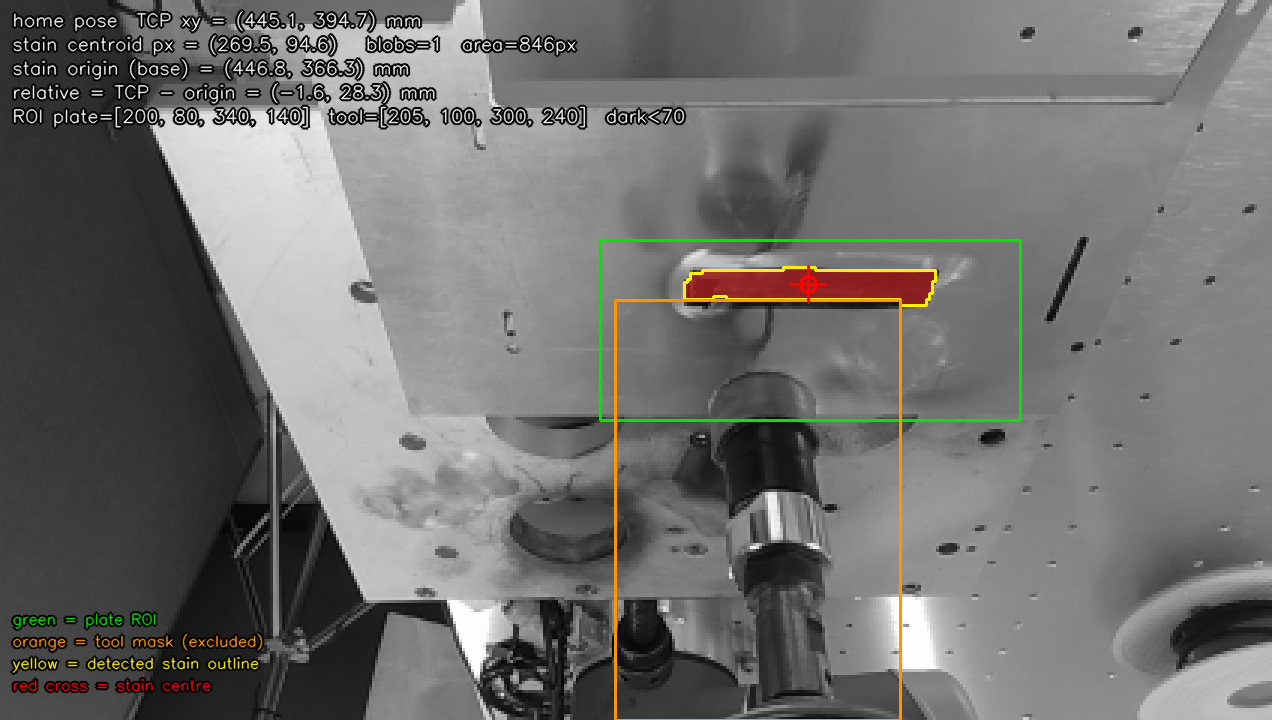
\includegraphics[width=0.87\linewidth]{figures/mark_detection_example.png}
\caption[Marked local region and registration]{Archived camera view of a marked local region and its registration overlay. The colored outlines belong to the existing detection display. This is an example of spatial instruction and image registration, not a validated micro-scratch detector or the fixed-origin E1 trial image.}
\label{fig:mark_example}
\end{figure}

The evaluated E1 comparison fixes \(c=(457.4,375.0)\) mm for all providers. Its evaluation band is specified independently by endpoints and width. The origin is a registration datum; it need not coincide with the midpoint of that band. In E2, the existing per-run origin interface is retained. Neither experiment uses a height-condition label as a policy input.

The policy's external stain-mask option is disabled for the evaluated checkpoints. Instead, the image encoder derives a fixed TCP interaction-region feature from RGB. The physical marking, the registered origin, the evaluator's spatial band, and the encoder's image ROI are therefore four different objects. Conflating them would incorrectly imply that the network is explicitly constrained to the evaluator's band or that it receives a segmentation of the complete processing strategy.

\section{Module Responsibilities}
Figure~\ref{fig:faire_architecture} shows the implemented path from human guidance to evaluation. A provider supplies a sequence, a common execution layer converts it into conditioned commands, and the lower-level controller produces the physical interaction. Measured robot pose and force provide feedback. Evaluation observes this interaction through its own procedural criteria.

\begin{figure}[tbp]\centering
\resizebox{\linewidth}{!}{%
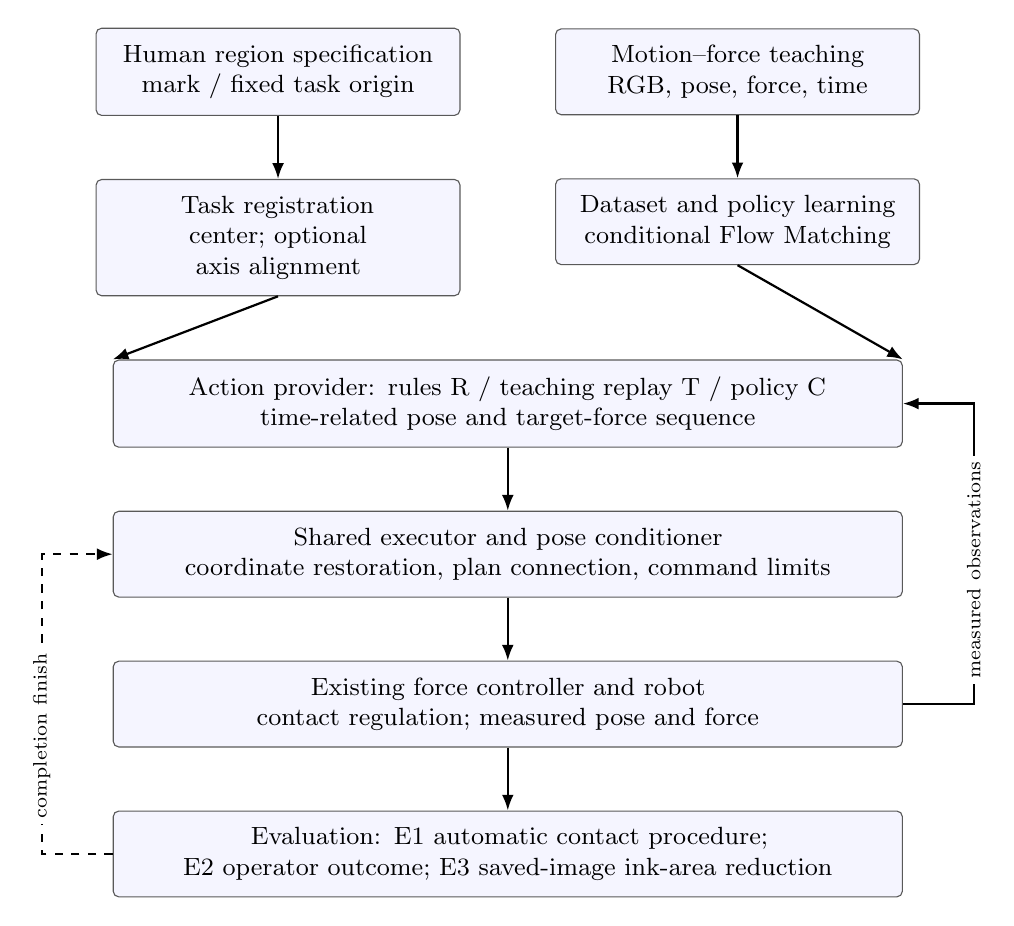
\begin{tikzpicture}[node distance=8mm]
\node[block,text width=42mm] (human) {Human region specification\\mark / fixed task origin};
\node[block,text width=42mm,right=12mm of human] (teach) {Motion--force teaching\\RGB, pose, force, time};
\node[block,text width=42mm,below=of human] (registration) {Task registration\\center; optional axis alignment};
\node[block,text width=42mm,below=of teach] (learning) {Dataset and policy learning\\conditional Flow Matching};
\node[block,text width=96mm,below=10mm of $(registration.south)!0.5!(learning.south)$] (provider) {Action provider: rules R / teaching replay T / policy C\\time-related pose and target-force sequence};
\node[block,text width=96mm,below=of provider] (exec) {Shared executor and pose conditioner\\coordinate restoration, plan connection, command limits};
\node[block,text width=96mm,below=of exec] (control) {Existing force controller and robot\\contact regulation; measured pose and force};
\node[block,text width=96mm,below=of control] (eval) {Evaluation: E1 automatic contact procedure;\\E2 operator outcome; E3 saved-image ink-area reduction};
\draw[link] (human)--(registration);\draw[link] (teach)--(learning);
\draw[link] (registration.south)--(provider.north west);
\draw[link] (learning.south)--(provider.north east);
\draw[link] (provider)--(exec);\draw[link] (exec)--(control);\draw[link] (control)--(eval);
\draw[link] (control.east)--++(9mm,0)|- (provider.east);
\node[rotate=90,font=\scriptsize,fill=white,inner sep=2pt]
 at ($(control.east)+(9mm,17mm)$) {measured observations};
\draw[link,dashed] (eval.west)--++(-9mm,0)|- (exec.west);
\node[rotate=90,font=\scriptsize,fill=white,inner sep=2pt]
 at ($(eval.west)+(-9mm,15mm)$) {completion finish};
\end{tikzpicture}}
\caption[System overview and module interfaces]{Implemented system overview. Solid arrows show data or execution flow. The dashed completion-to-executor arrow applies to E1's automatic finish/hold request; it does not synthesize an exit motion. E2 uses operator termination, and E3 removal is evaluated offline from saved photographs. The diagram is conceptual and editable.}
\label{fig:faire_architecture}
\end{figure}

\begin{table}[tbp]\centering\small
\caption[Module responsibilities]{Responsibilities of the human and system components.}
\label{tab:module_responsibilities}
\begin{tabularx}{\textwidth}{P{0.24\textwidth}X}
\toprule Component & Responsibility \\ \midrule
Human operator & Specify the local task, demonstrate motion and loading, set up the specimen, and provide recorded field observations. \\
Teaching system & Register tracked tool pose and record paired RGB, pose, force, and receipt-time evidence. \\
Skill provider & Supply a time-related reference sequence using a rule, a fixed demonstration, or a conditioned generator. \\
Common executor & Restore coordinates, interpolate references, connect plans, condition commands, and manage the existing finish/hold procedure. \\
Lower-level controller & Regulate physical contact using the supplied target force and measured state. \\
Task evaluator & Recognize E1's contact procedure, retain E2's operator outcome, or quantify E3's saved-image ink-area reduction under their separate definitions. \\
\bottomrule
\end{tabularx}
\end{table}

\section{Physical Platform and Observations}
The robot interface is the UR10 system identified by the deployed \texttt{ur10skku} topics and Cartesian command services. The teaching side uses a Vive tracker, calibrated tool pose, force/torque sensing, and a RealSense RGB stream. Robot execution records TCP pose from robot feedback and a processed six-axis wrench. The policy uses only the three force components. Torques remain useful logged diagnostics but are not policy inputs or actions for these checkpoints.

\begin{figure}[tbp]\centering
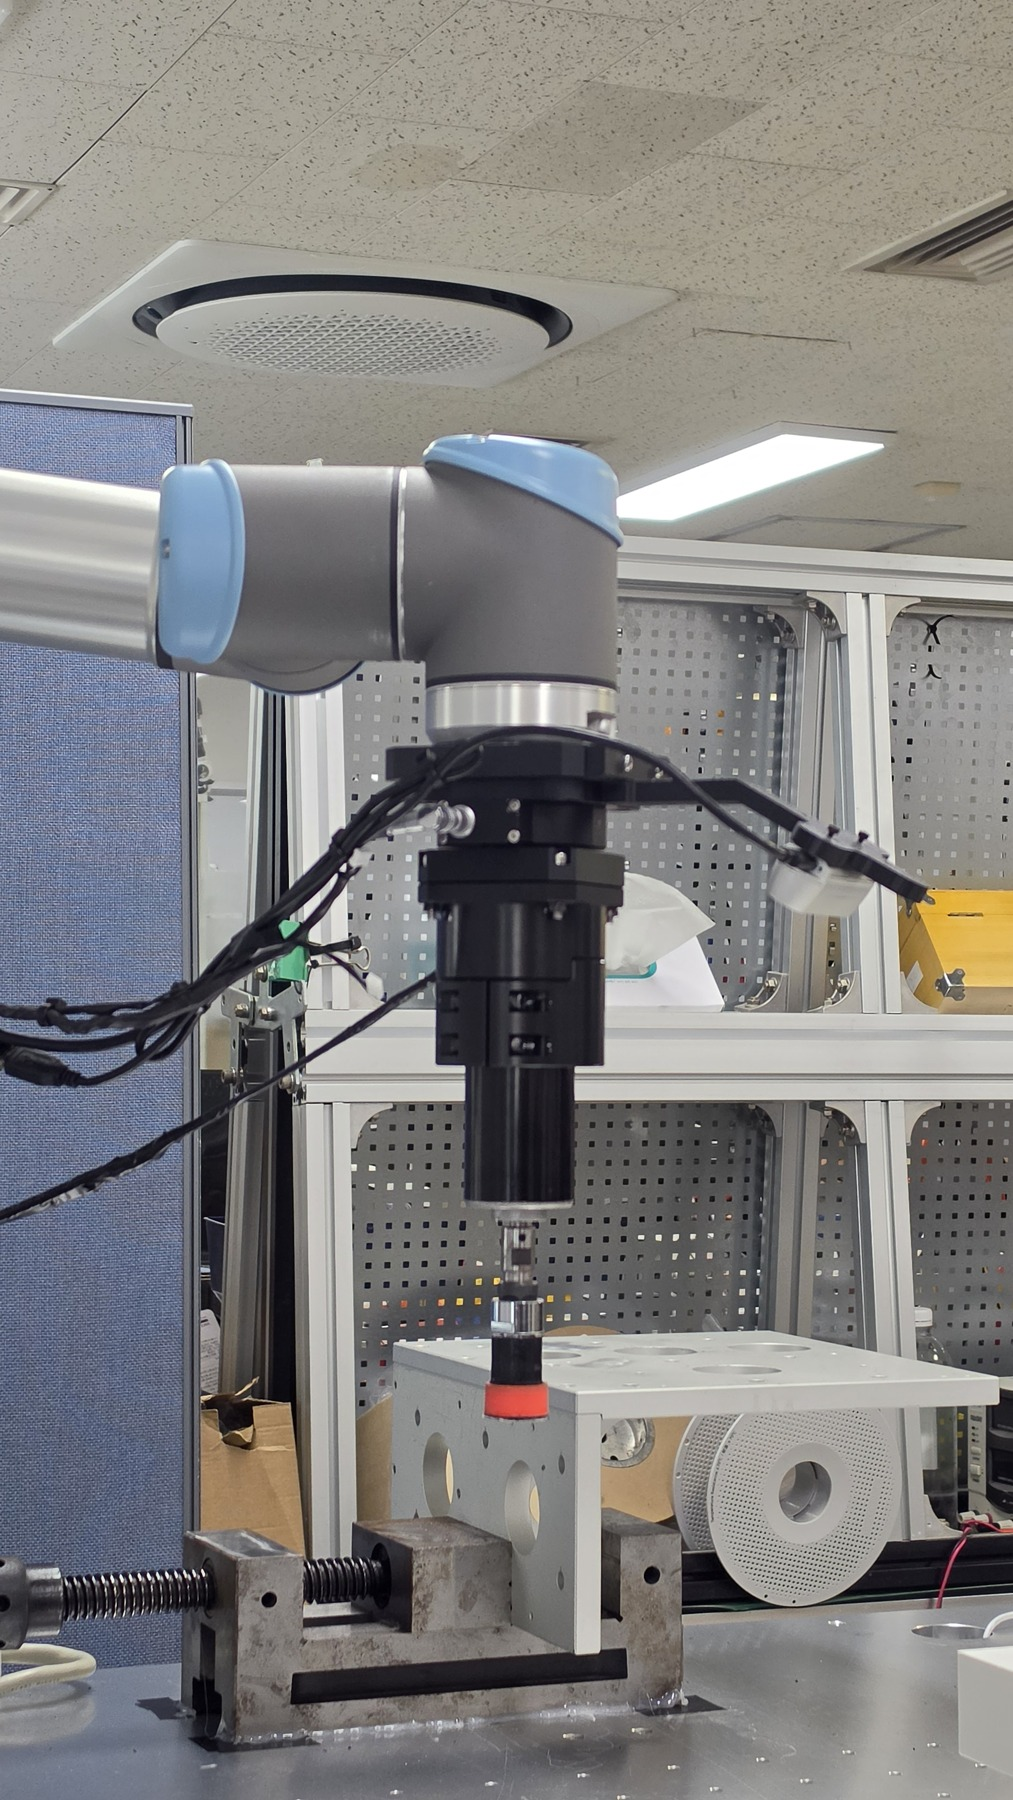
\includegraphics[width=0.67\linewidth,height=0.49\textheight,keepaspectratio]{figures/apparatus_20260807.jpg}
\caption[Archived robot apparatus photograph]{Genuine archived apparatus photograph dated 7 August 2026, showing the robot-mounted processing tool and fixture. Only image rotation and proportional resizing were applied. It illustrates the local experimental platform; it is not presented as a photograph taken during the October E1 or E2 runs.}
\label{fig:apparatus}
\end{figure}

The available records support a description of a robot-mounted local processing tool acting on a marked plate. They do not specify a complete process qualification, including measured spindle speed, material alloy, abrasive grade, or pre/post roughness. The experiments use measured robot interaction to answer procedural questions and E3 saved photographs to evaluate ink-area reduction. These limits do not prevent reproducing the learning and execution interfaces, but they restrict claims about manufacturing outcomes.

\section{Stain-Centered Learning and Direction Transfer}
\label{sec:stain_relative_generalization}
The representation separates the local movement pattern from its placement on the plate. Its training-data transformation expresses observation and action positions relative to a frozen stain center:
\begin{equation}
 \widetilde p_k=[p_{k,x}-c_x,\ p_{k,y}-c_y,\ p_{k,z}]^\mathsf{T},
 \qquad \widetilde\rho_k=\rho_k.
 \label{eq:relative_task_pose}
\end{equation}
This transformation retains the base-axis orientation and absolute Z coordinate. A single-direction demonstration consequently teaches a center-relative movement pattern in its original reference direction. The implementation additionally supports transferring that learned pattern to another in-plane stain direction through coordinated observation and action transformations. Training on centered positions and aligning directions at inference are two connected parts of the transfer mechanism; the dataset converter itself does not rotate the training episodes.

\subsection{Center and Axis from the Specified Region}
The reference-free registration path detects dark pixels within a configured plate area, excludes the tool area, and maps the retained pixels to robot-base XY coordinates using each image's pose-dependent planar homography. It pools these mapped points across the registration frames. Starting from their coordinate-wise median, four iterations retain the nearest 85\% of points and update the center by their mean. A singular-value decomposition of the trimmed, centered point cloud supplies the dominant strip axis. Its angle \(\theta_{\mathrm{live}}\in[0,\pi)\) is measured in base-plane radians. The axis is unoriented: the same strip has directions differing by \(\pi\), rather than an identified stroke-start endpoint.

The resulting center and optional angle are frozen together for the episode. An operator-supplied live angle is also supported. The direction therefore enters through explicit task registration rather than a learned output head. A center recovered from the visible mark identifies the intended task; it does not estimate defect depth or determine the desired force schedule.

\subsection{Observation Alignment and Path Restoration}
Let \(\theta_{\mathrm{ref}}\) denote the base-plane axis associated with the teaching reference direction. The implemented alignment angle and planar rotation are
\begin{align}
 \alpha&=\operatorname{wrap}_{\pi}
       (\theta_{\mathrm{ref}}-\theta_{\mathrm{live}}),
 &\operatorname{wrap}_{\pi}(\delta)
   &=((\delta+\pi/2)\bmod\pi)-\pi/2,\label{eq:stain_axis_alignment}\\
 R_2(\alpha)&=\begin{bmatrix}
  \cos\alpha&-\sin\alpha\\\sin\alpha&\cos\alpha
 \end{bmatrix}.&&\nonumber
\end{align}
The wrapped angle lies in \([-\pi/2,\pi/2)\). For an absolute measured XY position \(p_{k,xy}\), the policy-side position is
\begin{equation}
 u_k=R_2(\alpha)(p_{k,xy}-c).
 \label{eq:stain_canonical_observation}
\end{equation}
Center subtraction is applied first, followed by alignment to the teaching direction, and then by the checkpoint's numerical normalization. After the policy generates a sequence and the action bounds are inverted, each predicted XY position \(\widehat u_{k+j}\) is restored as
\begin{equation}
 p_{k+j,xy}^{\mathrm{ref}}
   =c+R_2(-\alpha)\widehat u_{k+j}.
 \label{eq:stain_canonical_action}
\end{equation}
The same inverse operation restores the stored demonstration-start XY pose before initial alignment. Thus both the live observation and generated path use the same frozen center and angle. Disabling direction alignment gives \(\alpha=0\) and reduces these equations to the translation-relative path used in E1/E2.

The single-camera policy image can also be rotated in plane about the configured TCP-ROI center, using the alignment angle and a configurable image-coordinate sign. The implementation uses bilinear image interpolation and reflected borders. This operation changes the image supplied to the policy while retaining the original view for recording and display. It adapts the visible direction to the reference view; a planar image rotation does not establish complete perspective or lighting invariance.

Only XY position is rotated by this adapter. Z, tool rotation-vector channels, target-force channels, and measured-force history retain their existing conventions. The method transfers a planar stroke direction while preserving the learned tool-posture and force interfaces; it is not a full rigid-frame transformation of pose and wrench. Its spatial role is distinct from observation-conditioned generation of the local motion--force sequence.

The current launch defaults leave direction alignment disabled. When enabled, the declared reference angle is \(132^\circ\), image rotation is enabled, and the maximum accepted alignment magnitude is \(65^\circ\). These are configurable reference and operating values, not a measured generalization range; the dataset name containing ``90deg'' is not used to infer the base-axis reference angle. If no live angle is available or the configured magnitude is exceeded, the implementation retains translation-only operation. Chapter~\ref{chap:demonstration_collection} distinguishes these implemented transfer operations from the particular dataset and settings used in the measured comparisons.

\section{Supported Conditions and Observable Success}
The E1/E2 datasets and runtime settings use center-relative XY coordinates with direction alignment disabled. E3 reuses the same C checkpoint and normalizer at registered planar placements, with observation XY/image alignment and generated XY inverse restoration enabled for D1/D2. Its position and direction changes are listed in Chapter~\ref{chap:experiments}; they describe task registration rather than independent precision surface metrology.

E1 defines observable success as contact formation, a continuous loaded ordered traversal of the fixed band, and a simultaneous unloaded upward exit. E2 uses the documented operator-based completion interpretation, corrected for the interrupted A4 attempt. E3 measures segmented board-marker ink-area reduction; image evaluability is independent of the automatic procedure label. These quantities are not pooled into one success statistic.

There is no learned termination output in the evaluated policy. A generated upward movement may reflect the demonstration's temporal structure. Recognition that the procedural exit has occurred belongs to the evaluator in E1 or to the operator's stopping decision in E2. Neither establishes that all defects have been removed. This distinction maintains a clear boundary between the generated skill and the state of the physical surface.

\chapter{Motion--Force Demonstration and Dataset Construction}
\label{chap:demonstration_collection}

\section{Teaching as a Source of Temporal Process Structure}
The purpose of teaching is to supply the motion and loading that remain unspecified by a local region. A demonstration records a tool's approach, motion through the working region, and departure together with the interaction force. This pairing supplies a temporal example for either direct replay or policy supervision. It does not include an independently measured defect-depth trajectory or a label that certifies material-removal completion.

The teaching system combines Vive tracking, a calibrated tool-pose publisher, force/torque sensing, and a RealSense RGB stream. The archived collection interface records six pose components and the first three force components. The paired data used by the evaluated models have a single RGB camera. Figure~\ref{fig:teaching_frames} shows actual frames from the selected replay episode's source, rather than a rendered apparatus or a substitute robot.

\begin{figure}[tbp]\centering
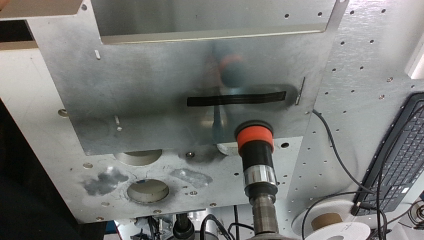
\includegraphics[width=.48\linewidth]{figures/teaching_ep29_frame000.png}\hfill
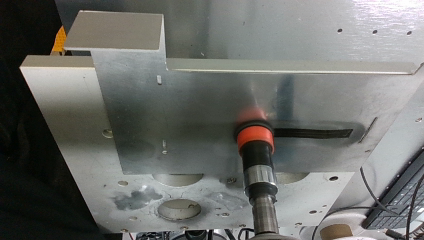
\includegraphics[width=.48\linewidth]{figures/teaching_ep29_frame085.png}\\[3pt]
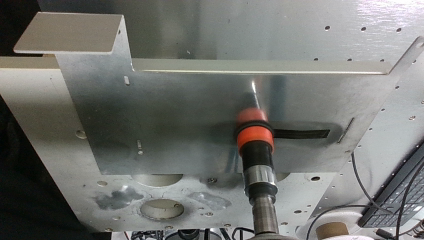
\includegraphics[width=.48\linewidth]{figures/teaching_ep29_frame150.png}\hfill
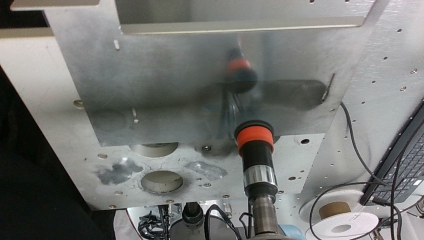
\includegraphics[width=.48\linewidth]{figures/teaching_ep29_frame400.png}
\caption[Actual teaching-camera frames]{Actual teaching-camera RGB frames associated with episode 29 at stored indices 0, 85, 150, and 400. The corresponding source is merged episode \texttt{ep\_0003}, recorded on 19 August 2026. The view shows the tool and marked plate during the recorded operation. It does not show the full tracker or sensor assembly.}
\label{fig:teaching_frames}
\end{figure}

\section{VR Registration and Tracker-to-Tool Conversion}
The recorded pose must refer to the tool rather than the tracker housing. Let \(V\) be the tracking frame, \(T\) the tracked rigid body, \(E\) the tool/TCP frame, and \(B\) the robot base. The nominal rigid coordinate chain is
\begin{equation}
 {}^BT_E(t)={}^BT_V\,{}^VT_T(t)\,{}^TT_E.
 \label{eq:demo_transfer}
\end{equation}
Figure~\ref{fig:demo_transfer} summarizes the coordinate-processing chain. The fixed transforms identify the tracking world with the robot base and remove the tracker-to-tool offset. Translation is expressed in millimeters, while the final orientation is converted to a rotation vector in radians.

The implementation includes more than one rigid transform. Its calibration utilities solve the registration and tool offset, project rotations to valid rotation matrices, and support a planar correction and a bounded XY-dependent position residual. The tracker publisher converts OpenVR translation from meters to millimeters before applying the downstream calibration chain. It right-multiplies the configured spatial-angle alignment and applies the selected tool-offset convention. The published \texttt{calibrated\_pose} is the final tool pose used by the recorder; the raw tracker rotation is not substituted for it in force-axis reconstruction.

The available calibration YAML records a 47-sample fit, planar correction, and a quadratic XY residual. Its stored residual RMS changes from 4.809 to 3.179 mm for that fit. These are calibration-fit diagnostics, not an independent accuracy test of every demonstration or October execution. The source also contains a configurable final constant offset. Consequently, a single conceptual frame-chain diagram is useful for understanding the registration, while the archived parameter file remains necessary for reproducing its numerical convention.

\begin{figure}[tbp]\centering
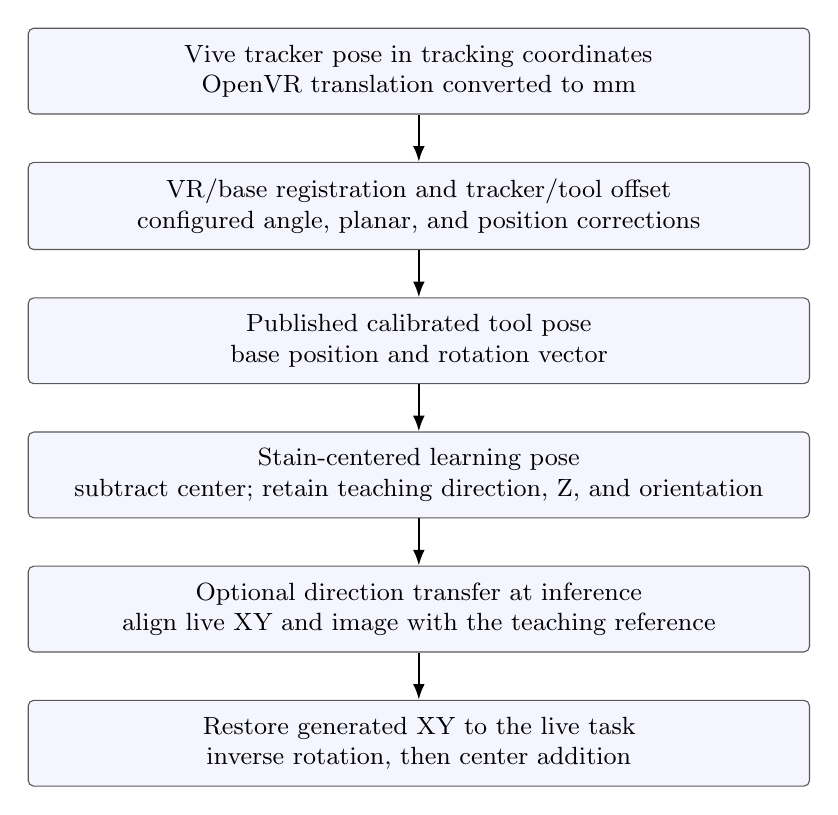
\begin{tikzpicture}[node distance=6mm]
\node[block,text width=95mm] (a) {Vive tracker pose in tracking coordinates\\OpenVR translation converted to mm};
\node[block,text width=95mm,below=of a] (b) {VR/base registration and tracker/tool offset\\configured angle, planar, and position corrections};
\node[block,text width=95mm,below=of b] (c) {Published calibrated tool pose\\base position and rotation vector};
\node[block,text width=95mm,below=of c] (d) {Stain-centered learning pose\\subtract center; retain teaching direction, Z, and orientation};
\node[block,text width=95mm,below=of d] (e) {Optional direction transfer at inference\\align live XY and image with the teaching reference};
\node[block,text width=95mm,below=of e] (f) {Restore generated XY to the live task\\inverse rotation, then center addition};
\draw[link](a)--(b);\draw[link](b)--(c);\draw[link](c)--(d);
\draw[link](d)--(e);\draw[link](e)--(f);
\end{tikzpicture}
\caption[Coordinate-processing and direction-transfer chain]{Implemented coordinate-processing roles, shown as an editable conceptual diagram. Calibration establishes the tool pose; center-relative learning and optional direction alignment register the local movement pattern. The last two boxes show the inference transfer in Equations~\eqref{eq:stain_canonical_observation} and~\eqref{eq:stain_canonical_action}, disabled in E1/E2 and enabled for the E3 direction conditions. Only XY positions are rotated; tool orientation and force channels retain their conventions.}
\label{fig:demo_transfer}
\end{figure}

\section{Synchronized Recording and the Meaning of Time}
The source merged HDF5 identifies its schema as multimodal synchronized recording, its master as camera 0, and its clock as subscriber-receive Unix time. The camera observation supplies the common sample time. Pose and force are associated through receive-time buffers, with a recorded maximum synchronization error parameter of 0.05 s. The archive retains the source times, interpolation indicators, and pose/force synchronization errors for each paired sample.

These timestamps describe software receipt and pairing. They are not hardware exposure timestamps or the original force-sensor acquisition times. Their value is that the construction of a paired sample is explicit and can be inspected. Their limitation is that transport delay and sensor latency cannot be removed simply by assigning all signals to one image time.

The representative source episode records a nominal 30 Hz grid, 443 paired frames, and the original \texttt{sample\_time\_unix} array. The compact learning file retains the paired images and signals but not that full time array. For the replay baseline and the teaching plots, the source episode is recovered using the compact file's \texttt{source\_h5} and \texttt{source\_episode} attributes. This preserves the actual paired time axis instead of reconstructing it solely from the nominal rate.

\section{Signal Stages and Force Processing}
The word raw depends on where a signal enters the pipeline. The recorder's \texttt{raw\_ft} is already a decoded and published measurement after the configured sign, startup-zero, and gravity-processing path. It is raw relative to the recorder's offline filter. It is not an uncorrected packet from the force sensor.

The teaching publisher applies its configured sensor decoding and sign convention, startup mean zeroing, selected publisher filtering, and delta-gravity compensation before publishing the wrench. The recorder then applies native-axis force filtering. In the representative archived episode, the force filter is an exponential moving average with \(\alpha=0.2\),
\begin{equation}
 \bar f_k=\alpha f_k+(1-\alpha)\bar f_{k-1}.
 \label{eq:force_ema}
\end{equation}
The stored pose is processed through the existing Hampel and difference-regularized smoothing pipeline. The archived episode reports no pose EMA, no approach slowdown, and retiming factor one. These are properties of the selected recorded episode; optional processing branches in the current recorder are not assumed to have been active.

Table~\ref{tab:signal_stages} distinguishes the recording, cleanup, and normalization stages.

\begin{table}[tbp]\centering\small
\caption[Teaching and learning signal stages]{Teaching and learning signal stages. Normalization changes scale for the network; it does not perform physical calibration.}
\label{tab:signal_stages}
\begin{tabularx}{\textwidth}{P{0.25\textwidth}X}
\toprule Stage & Meaning and use \\ \midrule
Published / recorder raw & Decoded and compensated force paired with calibrated pose; preserved as \texttt{raw\_ft} and \texttt{raw\_position}. \\
Filtered recording & Existing pose processing and force EMA; paired images and source-time mapping retained. \\
Learning cleanup & Derived force fields modified by the specified native-axis cleanup; pose and RGB preserved. \\
Normalized tensors & Training-split bounds map pose and force channels to the network scale. B then masks its force-conditioning tensors. \\
\bottomrule
\end{tabularx}
\end{table}

The 12 October force-cleanup dataset is a derived copy. It preserves the 42 episodes' images and pose fields, sets negative native \(F_z\) values to zero, and sets all three force components to zero where the associated stored \(z>175\) mm. Signed \(F_x,F_y\) remain unchanged in the other samples. The same rules apply to observation and action force fields. This height rule is an offline preprocessing convention tied to the stored coordinate system, not a new real-time contact detector or an estimate of material-removal depth.

Figure~\ref{fig:force_processing} shows these stages for the representative episode. Learning nonnegative targets does not impose a nonnegative output constraint on the generator. The archived model checks include negative unconditioned force predictions in some chunks; the runtime must therefore be described from its actual gating and command-processing code, rather than by assuming cleanup enforces a physical output bound.

\figfull{force_processing.pdf}{Actual force-processing stages for teaching episode 29. The upper panel compares post-publisher recorder raw force, offline EMA, and the learning cleanup in native axes. The lower panel rotates the complete cleanup force vector to robot-base axes using its paired tool orientation. These are different signal stages; none is a new physical calibration.}{fig:force_processing}

\section{Force Frames and Common-Axis Analysis}
The existing force correspondence analysis supplies a resolved relation between teaching published axes and the calibrated tool frame:
\begin{equation}
 R_{E\leftarrow\mathrm{pub}}=I,\qquad
 f_B(t)=R_{B\leftarrow E}(t)\,f_{\mathrm{pub,processed}}(t).
 \label{eq:normal_force_projection}
\end{equation}
The second relation is posture dependent. All three force components are rotated using the calibrated tool rotation. Sign, zero, and gravity corrections are already present in the published vector and are not applied again. Translating the XY task origin does not rotate force.

Robot feedback follows a different processing chain: startup zeroing, the archived moving-average stage, a fixed sensor-to-TCP rotation, TCP gravity correction, and TCP-to-base rotation before publication and copying into the current-force topic. The executor's recorded force is therefore already in robot-base axes. Re-rotating that CSV would be incorrect.

Common-axis reconstruction makes the recorded teaching distribution and measured robot-base component comparable for an empirical force-exposure statistic. It does not recover an unlogged controller-applied target or establish a force-tracking error. It also does not imply that training tensors were retrospectively rotated. The evaluated dataset keeps native teaching force, while the inference adapter reads the selected robot-force components directly before normalization. This numerical input convention is retained when reporting the actual evaluated implementation. A common-frame policy-training ablation was not performed.

\section{Relative Coordinates, Episodes, and Data Partitions}
The compact representation subtracts the stored stain center from observation and action XY positions, leaving Z and orientation unchanged. Learning this local pattern removes absolute XY placement from the pose supervision. The selected dataset is labeled single-direction, 90-degree, and explicitly records \texttt{rotation\_aligned=false}. This attribute describes the saved training data; it does not mean that the implementation lacks direction transfer. The separate inference adapter in Section~\ref{sec:stain_relative_generalization} aligns live positions and images to a configured teaching direction and inversely restores generated XY. E1/E2 explicitly disable that adapter, so their results do not quantify its transfer performance. Some upstream files also record episode-specific XYZ corrections, which are preprocessing transformations rather than separate generalization tests.

The evaluated A/B/C models share 42 unique episodes. The optimization partition contains 38 episodes; validation contains episodes 35, 39, 22, and 37. The checkpoint normalizer files reproduce this episode-level partition. All windows from an episode remain in its assigned partition, avoiding overlap of windows from one episode across optimization and validation. This does not establish independence by operator, material, specimen, or collection session. No separate held-out demonstration-test split is claimed.

Figure~\ref{fig:dataset_split} shows the episode lengths and fixed partition.

\figfull{dataset_split.pdf}{Stored lengths of all 42 episodes used by the force-cleanup models. Orange identifies the four validation episodes. The partition is made before window sampling; repeated windows are not independent demonstrations.}{fig:dataset_split}

The loader draws 50 start indices per episode and constructs a 128-step future sequence. End-of-episode padding repeats the final action and masks padded positions out of the loss. Force history includes the current sample and the preceding samples up to a length of 30; a short initial history is padded on the left with the first available value. Start sampling is resampled across training epochs. Its existing phase sampler upweights the one-second precontact period by five relative to free and contact periods, using the recorded force thresholds of 3.0 and 1.2 N. The offline sampler uses this force-derived phase information for all three conditions, including A. A's policy still receives no force observation or force target.

Normalization bounds are computed from optimization-training episodes only. For channel \(d\), the implemented min--max mapping is
\begin{equation}
 \mathcal N_d(x)=2\frac{x-m_d}{\max(M_d-m_d,\epsilon)}-1,
 \label{eq:minmax_normalization}
\end{equation}
where \(m_d,M_d\) are the stored training bounds and \(\epsilon\) is the numerical denominator floor. State and action bounds are stored separately; force history uses the state-force bounds. Normalization does not force all future online values to lie within the training range.

\section{A Representative Motion--Force Pairing}
Episode 29 is used to explain the temporal representation because it is the operator-selected replay source, rather than an episode chosen for low error. Figure~\ref{fig:teaching_motion_force} presents its actual position and force history. The transition from approach to loaded movement and then rising motion gives a structured association between location, loading, and time. Replay uses that association directly; learning uses many such future windows as supervision.

\figfull{teaching_motion_force.pdf}{Teaching episode 29 on the original paired source-time axis. XY is task relative, Z remains in the stored absolute convention, and force is the native-axis cleanup signal. The 175 mm line is the offline cleanup boundary. The curves are not a desired-versus-measured robot force-tracking comparison.}{fig:teaching_motion_force}

The force action derives from measured teaching interaction, not an independently recorded human command. Physical equivalence must be assessed from robot measurements because the mechanics and controller differ.

\chapter{Force-Conditioned Motion--Force Skill Learning}
\label{chap:force_il}

\section{Learning Objective and Observation Interface}
The learning problem is to generate a future local skill from the execution context, while preserving a joint representation of movement and target loading. A conditioned sequence can change at a later inference call when the robot reaches a different pose or contact state. The policy is not asked to estimate scratch depth, choose an abrasive, or output a separate completion decision.

For the force-observing model, the physical observation at index \(k\) is
\begin{equation}
 o_k=\left(I_k,\widetilde q_k,f_k^{\mathrm{meas}},
       f_{k-L+1:k}^{\mathrm{meas}}\right),\qquad L=30.
 \label{eq:il_observation}
\end{equation}
The numerical state has nine components: six Cartesian pose values and three current force values. History has shape \(30\times3\). Only \(F_x,F_y,F_z\) enter this observation; the sensor's torque channels do not. The input image is the single \(240\times424\) RGB view. Images are converted to floating-point tensors and normalized using the implemented RGB channel means and standard deviations.

The action target is a normalized \(128\times9\) sequence of task-relative position, rotation vector, and teaching-derived target force. Position and orientation describe the tool reference, whereas force describes a controller-level target. Both appear in the same sequence so that their temporal correspondence can be learned. The action horizon corresponds to approximately 4.27 s on the nominal 30 Hz action grid. Its last sample is at \(127/30\) s relative to the first, which distinguishes a sample count from an endpoint-to-endpoint duration.

\section{Implemented Observation Encoder}
The active model is the Flow RGB policy in the archived training snapshot. It uses a frozen DINOv3 ViT-small patch-16 image backbone, a state MLP, a one-layer force-history GRU, and a fusion MLP. The separate encoder modules available elsewhere in the repository do not determine this checkpoint's architecture.

The visual branch combines the global image feature with a feature pooled from a fixed TCP interaction ROI. The ROI is constructed internally from reference image dimensions \(424\times240\), center \((253,120)\), and area-fraction parameter 0.25. The DINO patch features in that ROI are pooled by the configured attention mechanism. Global and ROI features are each projected to 512 components. The ROI is a calibrated interaction-region prior, not an external defect mask and not a prediction of surface damage.

The state MLP encodes all nine normalized state components into 256 components. A GRU with input dimension three and hidden dimension 64 encodes the force history, with its final hidden state contributing to fusion. The fused condition is 256-dimensional. Thus the current force appears both in the state vector and as the last history sample. There is no learned moment-history branch, LSTM comparison, or termination head in the evaluated configuration.

\begin{figure}[tbp]\centering
\resizebox{\linewidth}{!}{%
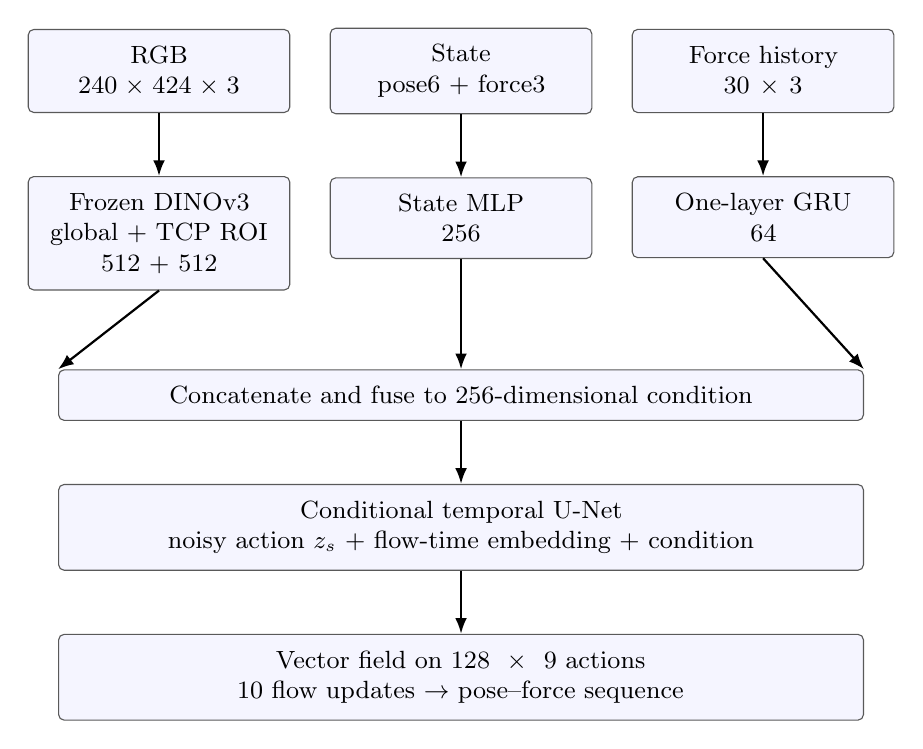
\begin{tikzpicture}[node distance=8mm]
\node[block,text width=29mm] (rgb) {RGB\\$240\times424\times3$};
\node[block,text width=29mm,right=5mm of rgb] (state) {State\\pose6 + force3};
\node[block,text width=29mm,right=5mm of state] (history) {Force history\\$30\times3$};
\node[block,text width=29mm,below=of rgb] (visual) {Frozen DINOv3\\global + TCP ROI\\$512+512$};
\node[block,text width=29mm,below=of state] (mlp) {State MLP\\256};
\node[block,text width=29mm,below=of history] (gru) {One-layer GRU\\64};
\node[block,text width=98mm,below=14mm of mlp] (fuse) {Concatenate and fuse to 256-dimensional condition};
\node[block,text width=98mm,below=of fuse] (unet) {Conditional temporal U-Net\\noisy action $z_s$ + flow-time embedding + condition};
\node[block,text width=98mm,below=of unet] (out) {Vector field on $128\times9$ actions\\10 flow updates $\rightarrow$ pose--force sequence};
\draw[link](rgb)--(visual);\draw[link](state)--(mlp);\draw[link](history)--(gru);
\draw[link](visual.south)--(fuse.north west);\draw[link](mlp)--(fuse);\draw[link](gru.south)--(fuse.north east);
\draw[link](fuse)--(unet);\draw[link](unet)--(out);
\end{tikzpicture}}
\caption[Implemented policy architecture]{Actual force-observing policy configuration, shown conceptually. In B, the current-force and history tensors are zeroed after normalization while the history branch remains. A uses pose6 state/action and omits force history. The flow vector field has the same sequence shape as its action input.}
\label{fig:force_history_policy}
\end{figure}

\begin{table}[tbp]\centering\small
\caption[Architecture and training settings]{Architecture and training settings for the force-cleanup checkpoints used in E1--E3.}
\label{tab:learning_settings}
\begin{tabularx}{\textwidth}{P{0.48\textwidth}X}
\toprule Item & Stored value \\ \midrule
Backbone / trainable status & DINOv3 ViT-small, patch 16 / frozen \\
State / history / global condition & 256 / 64 / 256 components \\
Temporal U-Net channel widths & 256, 512, 1024 \\
Convolution kernel / groups & 5 / 8 \\
Flow-time embedding & 256 components \\
Action horizon / force-history length & 128 / 30 samples \\
Loss / flow integration updates & Masked MSE / 10 \\
Optimizer & AdamW, learning rate \(10^{-4}\) \\
Weight decay / optimizer betas & \(10^{-5}\) / \((0.95,0.999)\) \\
Batch size / training seed & 12 / 0 \\
Training epochs / warmup & 500 / 10 epochs \\
Learning-rate schedule & Cosine; minimum \(10^{-6}\) \\
Gradient norm clip & 1.0 \\
\bottomrule
\end{tabularx}
\end{table}

\section{Flow Matching Sample Construction}
Flow Matching learns a field that transports a simple noise distribution toward the demonstrated sequence distribution~\cite{lipman2023flow}. The following equations describe the particular implemented construction, rather than all possible flow-matching paths.

Let \(A\in\R^{H\times d_a}\) be a demonstrated action chunk after action normalization, with \(d_a=9\) for B/C and \(d_a=6\) for A. Independently sample a noise chunk \(Z_0\sim\mathcal N(0,I)\) with the same shape and a scalar flow time
\begin{equation}
 s\sim\mathcal U(\varepsilon,1-\varepsilon),\qquad\varepsilon=10^{-4}.
\end{equation}
The source implementation uses
\begin{equation}
 Z_s=(1-s)Z_0+sA,\qquad U=A-Z_0.
 \label{eq:flow_training_path}
\end{equation}
The vector-field network \(v_\theta(Z_s,s,c_k)\) predicts \(U\), conditioned on the encoded observation \(c_k=E_\theta(o_k)\). The scalar \(s\) belongs to a dimensionless generative process. It is unrelated to the physical polishing time \(t\) or the future sample index \(j\).

Let \(m_j\) equal one when future step \(j\) has actual episode support and zero when it is padded. The implemented per-batch objective is
\begin{equation}
 \mathcal L_{\mathrm{FM}}=
 \frac{\displaystyle\sum_{b,j,d}m_{bj}
 \left[v_\theta(Z_{s_b},s_b,c_b)_{jd}-(A_b-Z_{0,b})_{jd}\right]^2}
 {d_a\,\max\!\left(1,\sum_{b,j}m_{bj}\right)}.
 \label{eq:imitation_loss}
\end{equation}
Here \(b\) indexes batch elements, \(j\) future action steps, and \(d\) action coordinates. A new noise tensor and flow time are sampled for the training evaluation. All valid normalized coordinates contribute to the same MSE. There are no additional orientation-geodesic, target-force-tracking, material-removal, or completion losses in this configuration.

The conditional temporal U-Net operates along the action-sequence dimension. Its residual blocks combine temporal convolutions with the global observation and flow-time condition. The configured channel levels are 256, 512, and 1024; convolutional blocks use GroupNorm and Mish nonlinearities. These choices parameterize the field rather than creating a separate head for each physical objective. In particular, a lower force-related loss is not computed independently from the motion coordinates.

\section{Flow Integration and Physical Timing}
At inference, a fresh Gaussian chunk \(Z^{(0)}\) is generated. With \(M=10\) and \(h=1/M\), the source applies
\begin{equation}
 Z^{(m+1)}=Z^{(m)}+h\,
 v_\theta\!\left(Z^{(m)},(m+\tfrac12)h,c_k\right),
 \quad m=0,\ldots,M-1.
 \label{eq:flow_integration}
\end{equation}
This is the exact explicit update with a midpoint flow-time argument used in the code. It is not a two-stage midpoint Runge--Kutta solver: no intermediate state evaluation is computed. The final sequence is denormalized using the stored action bounds, and its relative XY coordinates are restored before execution. When the implemented direction-transfer option is active, observation XY and the single-camera policy image are aligned before conditioning, and generated XY is inversely rotated before center addition, as defined in Section~\ref{sec:stain_relative_generalization}. This adapter surrounds the learned generator without changing its training objective or adding a predicted direction channel. It is disabled in E1/E2 and enabled for the E3 direction conditions.

Ten flow updates generate an entire chunk. They are not ten physical polishing steps, and the physical action grid does not run at the flow-integration frequency. Online generation is triggered through a 5 Hz inference timer but is gated by existing plan age: the nominal stride is 120 samples at 30 Hz, or four seconds of reference progression. The actual recorded calls are separated by timer scheduling and inference latency as well. This gives observation-conditioned replanning at chunk boundaries, not a claim of continuous high-frequency strategy correction.

The force history also has two time interpretations. In the dataset, 30 samples on a nominal 30 Hz grid describe approximately one second of historical context. Online, the adapter retains the most recent 30 force callback values and left-pads an insufficient history; it does not resample them onto an exact one-second clock. A 20 Hz recording cap for diagnostic CSV files does not specify the policy callback rate. The history length is therefore reported as a sample count, with its nominal training duration stated separately.

\section{Separating Force Output from Force Observation}
The three E2 conditions implement different information contracts. A has a six-dimensional pose state and six-dimensional pose action, with no force-history encoder or force supervision. An external constant 23 N target is supplied by the execution interface; it is not an A policy output. B retains the nine-dimensional action and the same history architecture as C, but the current-force part of its normalized state and its normalized history tensor are replaced by zeros. C retains the measured-force inputs.

Masking occurs in the dataset/model conditioning path during training and again at the inference boundary. It does not alter the force-action target. Because masking is applied after normalization, a zero conditioning value is a neutral network input, not a declaration that physical measured force is zero newtons. B remains a separately trained model. It uses the same teaching episodes and retains their force-action targets, learning a target-force sequence conditioned on image and pose even though measured force is masked at its observation input. It is not C evaluated after an untrained removal of its inputs.

The title's two terms identify these separate roles. \emph{Joint motion--force representation} pairs pose and teaching-derived target force on the same action time axis. \emph{Force-conditioned imitation learning} additionally uses current measured force and force history as observation conditioning. The force coordinates of a noisy action chunk in Equation~\eqref{eq:flow_training_path} are part of the generative training path, not observed force inputs. Table~\ref{tab:e2_information_contracts} and Figure~\ref{fig:e2_information_flow} make the distinction explicit.

\begin{table}[tbp]\centering\footnotesize
\caption[E2 input, supervision, and external target]{Information contracts for three separately trained conditions using the same 42 episodes (38 training, four validation). Pose denotes tool position and orientation. All conditions retain actual force feedback in the lower-level controller.}
\label{tab:e2_information_contracts}
\begin{tabularx}{\linewidth}{lP{.34\linewidth}P{.23\linewidth}X}
\toprule Model & Policy observation & Action supervision & Force reference \\ \midrule
A & \(I_t,\mathrm{pose}_t\) & \(\mathrm{pose}_{t:t+127}\) & External 23 N \\
B & \(I_t,\mathrm{pose}_t,0,0_{30\times3}\) & \((\mathrm{pose},f^{\mathrm{target}})_{t:t+127}\) & Policy force output \\
C & \(I_t,\mathrm{pose}_t,f^{\mathrm{meas}}_t,\mathcal H_t\) & \((\mathrm{pose},f^{\mathrm{target}})_{t:t+127}\) & Policy force output \\
\bottomrule
\end{tabularx}
\end{table}

Here \(\mathcal H_t=f^{\mathrm{meas}}_{t-29:t}\); B's zeros replace normalized conditioning tensors and do not mean a physical reading of 0 N. At a selected training index, the current RGB/pose observation and supported force history condition the future 128-sample action chunk. Samples beyond the episode end are padded and excluded by the existing loss mask. This explanatory notation summarizes sample construction; the actual objective remains the masked flow-vector-field loss in Equation~\eqref{eq:imitation_loss}.

\begin{figure}[tbp]\centering
\resizebox{\linewidth}{!}{%
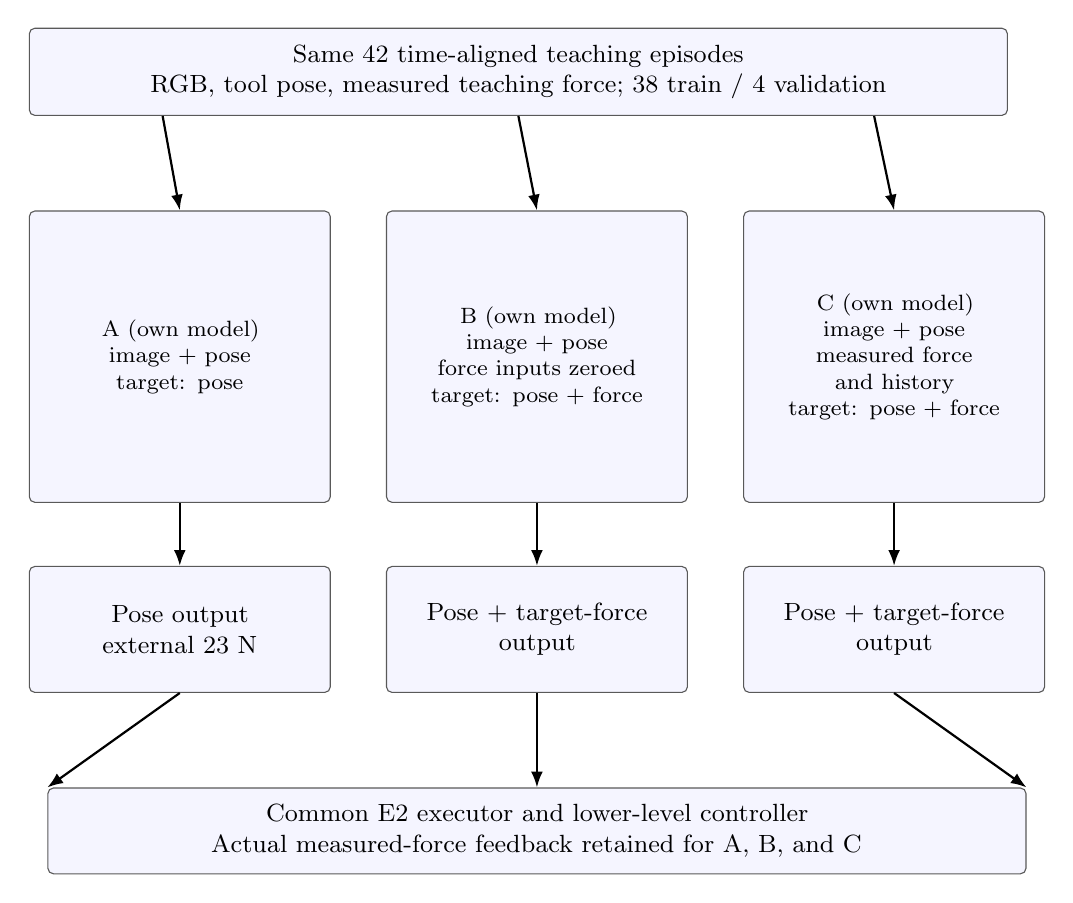
\begin{tikzpicture}[node distance=8mm]
\node[block,text width=120mm] (data) {Same 42 time-aligned teaching episodes\\RGB, tool pose, measured teaching force; 38 train / 4 validation};
\node[block,text width=34mm,font=\footnotesize,minimum height=37mm,below=12mm of data.south west,anchor=north west] (a) {A (own model)\\image + pose\\target: pose};
\node[block,text width=34mm,font=\footnotesize,minimum height=37mm,right=7mm of a] (b) {B (own model)\\image + pose\\force inputs zeroed\\target: pose + force};
\node[block,text width=34mm,font=\footnotesize,minimum height=37mm,right=7mm of b] (c) {C (own model)\\image + pose\\measured force\\and history\\target: pose + force};
\node[block,text width=34mm,minimum height=16mm,below=8mm of a] (ao) {Pose output\\external 23 N};
\node[block,text width=34mm,minimum height=16mm,below=8mm of b] (bo) {Pose + target-force\\output};
\node[block,text width=34mm,minimum height=16mm,below=8mm of c] (co) {Pose + target-force\\output};
\node[block,text width=120mm,below=12mm of bo] (exec) {Common E2 executor and lower-level controller\\Actual measured-force feedback retained for A, B, and C};
\draw[link](data.south west)++(17mm,0)--(a.north);
\draw[link](data.south)--(b.north);
\draw[link](data.south east)++(-17mm,0)--(c.north);
\draw[link](a)--(ao);\draw[link](b)--(bo);\draw[link](c)--(co);
\draw[link](ao.south)--(exec.north west);\draw[link](bo)--(exec);\draw[link](co.south)--(exec.north east);
\end{tikzpicture}}
\caption[E2 force-information learning and execution]{Explanatory information-flow diagram. B/C have the same motion--force supervision and architecture; B masks only normalized force conditioning in training and inference. Each condition has its own trained checkpoint. The shared lower-level measured-force feedback is preserved.}
\label{fig:e2_information_flow}
\end{figure}

The force signal is still used by the common executor and lower-level controller in A and B. It is also used by the existing offline phase sampler. Thus ``force observation OFF'' refers specifically to the policy's conditioning channels. Chapter~\ref{chap:experiments} uses this distinction to interpret the A/B comparison as a force-output comparison and B/C as a force-observation comparison, subject to the limitations of separate single-seed training.

\section{Training Completion and Checkpoint Selection}
The recorded training completed 500 epochs per condition, ending at zero-based epoch 499. The deployed best checkpoints are selected by minimum validation loss, as confirmed by both the model manifest and the checkpoint metadata. Table~\ref{tab:checkpoints} distinguishes the configured duration from the selected epoch.

\begin{table}[tbp]\centering\small
\caption[Selected checkpoint epochs]{Selected checkpoints. Epoch values follow the stored zero-based convention. Validation losses have different action dimensions for A versus B/C and are not task-performance scores.}
\label{tab:checkpoints}
\begin{tabular}{lrrrr}
\toprule Model & State/action dim. & Best epoch & Final epoch & Best val. loss \\ \midrule
A & 6 / 6 & 39 & 499 & 0.049722 \\
B & 9 / 9 & 42 & 499 & 0.069948 \\
C & 9 / 9 & 42 & 499 & 0.066444 \\
\bottomrule
\end{tabular}
\end{table}

Validation evaluates the same flow-field objective using held-out episodes. Its minimum selects a generative model according to that objective, not according to robot task completion or measured finish quality. Since noise and flow time enter the loss evaluation, the numerical minimum also should not be interpreted as a deterministic physical optimum. There is one recorded training seed per condition. Five robot repetitions per condition evaluate execution of that trained model; they do not constitute five independently trained policies.

The resulting method offers a concrete mechanism for coupling motion and target loading under observations. Whether the mechanism improves a given local task remains an empirical question. Its demonstrated function is generation and deployment of the specified action representation; its broader value is assessed alongside rules and replay in the following chapters.

\chapter{Robot Execution and Contact-Task Evaluation}
\label{chap:execution}

\section{From a Skill Sequence to Robot Commands}
Figure~\ref{fig:execution_architecture} summarizes the command-processing chain.
The generated sequence is an upper-level reference. Its physical meaning depends on the execution system that samples it, connects new plans, gates force, and transmits commands to the existing controller. A common execution layer is therefore necessary for interpreting differences between providers.

The provider interface supplies a time array, pose--force values, a plan identifier, and whether the plan is finite. R supplies a prescribed finite path with a recipe force. T supplies a finite teaching sequence with its original time axis. C supplies successively generated chunks from observations. Relative XY positions are restored using the frozen task origin before commands are interpreted in robot-base position coordinates. In the optional direction-transfer path, inverse XY rotation precedes that addition; the evaluated E1/E2 configuration uses translation alone. This restoration occurs before downstream command conditioning. The accompanying force values remain controller targets, with their frame interpreted by the lower-level configuration.

The timed sampler uses elapsed reference time rather than selecting the closest spatial waypoint. It linearly interpolates position and force and interpolates orientation on \(SO(3)\). This preserves the association between a source time and its requested pose/force. It does not guarantee identical physical feed velocity, because downstream conditioning and contact dynamics can alter motion.

\section{Shared Pose Conditioning and Plan Connection}
The evaluated E1 configuration applies the same archived pose conditioner to R, T, and C. Earlier metadata within the profile still refers to its initial C-only introduction; the active shared R/T/C wrapper and recorded runtime establish the later comparison's actual scope. R/T are presented through a private 30 Hz, 128-point pose view with a 120-point stride, while their original finite force/time plans remain the source for force sampling and phase boundaries.

The conditioner smooths XYZ with a 35-point moving average and orientation with a quaternion mean. The latter avoids averaging rotation vectors through their branch cut near \(\pi\). Edge padding is confined to the filter's window construction. A replacement plan is joined to the preceding reference and velocity over 0.5 s. Its quintic connection weight is
\begin{equation}
 \beta(u)=10u^3-15u^4+6u^5,\qquad
 u=\min(1,(t-t_b)/0.5),
 \label{eq:plan_connection}
\end{equation}
where \(t_b\) is the connection start. Position connects from a velocity-extended anchor; orientation uses a bounded relative rotation. The conditioner also retains its velocity state across replacement plans and bounds the change in commanded velocity.

These operations alter the reference actually presented to the command loop. They are shared processing choices, rather than evidence that the generated raw chunks are intrinsically smooth. Likewise, T's time scaling of one describes its source-time replay, not equality between the demonstrator's and robot's measured instantaneous speed.

\begin{figure}[tbp]\centering
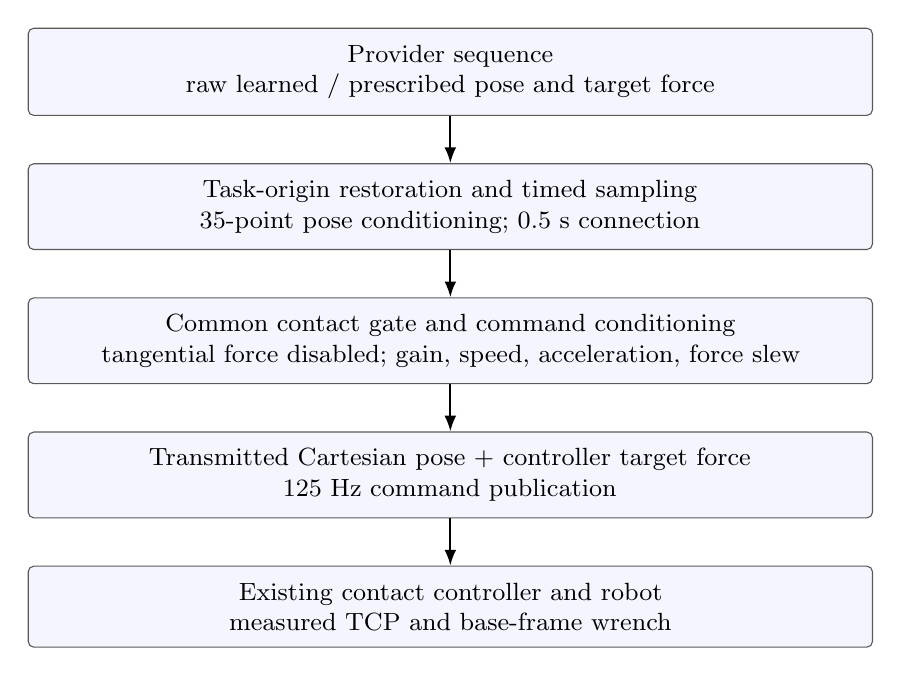
\begin{tikzpicture}[node distance=6mm]
\node[block,text width=103mm] (p) {Provider sequence\\raw learned / prescribed pose and target force};
\node[block,text width=103mm,below=of p] (c) {Task-origin restoration and timed sampling\\35-point pose conditioning; 0.5 s connection};
\node[block,text width=103mm,below=of c] (g) {Common contact gate and command conditioning\\tangential force disabled; gain, speed, acceleration, force slew};
\node[block,text width=103mm,below=of g] (s) {Transmitted Cartesian pose + controller target force\\125 Hz command publication};
\node[block,text width=103mm,below=of s] (l) {Existing contact controller and robot\\measured TCP and base-frame wrench};
\draw[link](p)--(c);\draw[link](c)--(g);\draw[link](g)--(s);\draw[link](s)--(l);
\end{tikzpicture}
\caption[Command processing and contact execution]{Execution interface and distinct command stages. The transmitted target is observable in executor logs; the controller-applied target is not available as a synchronized time series. This conceptual diagram describes command processing, not measured force-tracking performance.}
\label{fig:execution_architecture}
\end{figure}

\section{Command Rates, Limits, and Force Gating}
The command loop uses a nominal 0.008 s period, corresponding to 125 Hz. The common proportional command-update gain is 15 s\(^{-1}\), with per-axis position speed cap 10 mm/s and angular cap 40 degrees/s. The pose-conditioning acceleration settings are 25 mm/s\(^2\) and 100 degrees/s\(^2\). The force-command slew limit is 30 N/s. These are command-processing settings, not experimentally measured limits of physical tool speed or contact force.

For a scalar translational component, the shared update can be represented as
\begin{equation}
 \delta x_i=\operatorname{clip}\bigl(\min(1,K\Delta t)(x_i^\star-x_i^{\mathrm{cmd}}),
                    -v_i^{\max}\Delta t,v_i^{\max}\Delta t\bigr),
 \label{eq:command_update}
\end{equation}
followed by the existing acceleration conditioning. \(x_i^\star\) is the sampled conditioned reference, \(K=15\) s\(^{-1}\), and \(\Delta t\) is bounded by the nominal control period. Orientation uses a relative-rotation increment instead of direct component-wise interpolation across a branch cut.

The operational gate reads measured robot-base \(F_z^B\), enters contact at 3.0 N, and leaves at 1.2 N. While the gate is OFF, the requested normal target is suppressed. The command's tangential force components are set to zero in the evaluated common executor. Thus B/C learn a three-component force action, but the deployed comparison transmits only its normal-force component as a nonzero target. Their three-component measured-force observations can still inform generation.

The target's final approach to its requested value is affected by gain and slew conditioning. A nominal constant recipe is therefore distinct from the full transmitted force curve, particularly around contact onset and release. In E1, R uses 18 N. In E2, A uses an external 23 N target. The operator's approximate 20 N teaching intention, those recipe values, and the measured base-force distribution describe different quantities.

\section{Existing Lower-Level Contact Regulation}
The archived controller receives a Cartesian pose reference and a signed target-force vector. Its TCP-coordinate path rotates measured base vectors into the local frame, performs contact-control computation there, and restores the resulting motion to the robot frame. The stored controller configuration identifies TCP force coordinates and an existing mass/damping adaptation mode. This lower-level adaptation is a shared control asset; it is not the upper-level residual surface-repair policy proposed in the old thesis.

The underlying admittance implementation defines position error \(e=x_d-x_c\) and force error \(F_d-F_{\mathrm{ext}}\). Its scalar virtual dynamics can be written as
\begin{equation}
 M\ddot e+D\dot e+Ke=F_d-F_{\mathrm{ext}},\qquad x_c=x_d-e,
 \label{eq:admittance_il}
\end{equation}
where \(x_d\) is the supplied motion reference, \(x_c\) the compliant motion output, and \(M,D,K\) the virtual mass, damping, and stiffness. This controller calculation converts position to meters internally; its translational parameter units are kg, N\,s/m, and N/m. The source discretizes the relation using the Tustin form and contains mode-dependent parameter updates. Equation~\eqref{eq:admittance_il} explains the interaction role; it does not replace the deployed switching and adaptation logic with a newly designed controller.

Teaching force, policy output, transmitted target, and measured force must remain distinct. The available axis correspondence permits rotating teaching measurements into robot-base coordinates for analysis. It does not provide the actual controller-applied reference after all internal processing. For that reason, the thesis does not subtract published TCP target \(F_z\) directly from measured base \(F_z\) and call the result tracking RMSE.

\section{Approach and Contact-Start Synchronization}
R and T retain an existing one-time contact-start synchronization. Before confirmed contact, their approach reference continues to progress up to the prescribed processing boundary. Once distinct received force observations sustain the existing ON state for 0.2 s, the reference clock is aligned to that boundary. After the alignment, the finite strategy advances from its source timing; repeated synchronization is not applied.

This mechanism matters because the physical surface can be encountered before or after a nominal geometric boundary. It supplies feedback to fixed strategies without learning a policy. C instead generates its own approach and later chunks from observations. Common contact gating and lower-level force regulation remain active in all methods.

The normal departure is also provider dependent. R includes a planned zero-force upward segment, T contains the selected teaching exit, and C can generate an exit within its pose--force sequence. The evaluator recognizes the result of these actions. It does not insert a new retraction to make a deficient sequence satisfy the task.

\section{The Executed E1 Contact Procedure}
E1 uses a fixed 25 mm-wide XY band between \(P_0=(445,395)\) mm and \(P_1=(487,345)\) mm. Its length is 65.299 mm and it is divided into 14 longitudinal segments. The band concerns the TCP center; it is not a measurement of the contact footprint.

Let \(d=(P_1-P_0)/\ell\), \(\ell=\|P_1-P_0\|\), and let \(n\) be a unit vector perpendicular to \(d\) in the XY plane. For TCP XY position \(p_{xy}\), define longitudinal and transverse coordinates
\begin{equation}
 u=d^\mathsf{T}(p_{xy}-P_0),\qquad
 v=n^\mathsf{T}(p_{xy}-P_0).
 \label{eq:task_band}
\end{equation}
Band occupancy requires \(0\leq u\leq\ell\) and \(|v|\leq12.5\) mm. An ordered loaded candidate starts at an end segment and advances through adjacent first visits toward the opposite end. Contact OFF, missing support, or leaving the band breaks a candidate. Revisiting a previously visited segment does not create additional forward progress. Completion of the 14-segment sequence establishes the required pass. There is no per-segment 0.466 s dwell requirement in this primary criterion.

The primary E1 session uses \texttt{pass\_height\_ref\_v2}. The evaluator first confirms contact for 0.2 s. Once the first continuous loaded ordered pass succeeds, it freezes the working-height reference \(z_{\mathrm{work\_ref}}\). This is the time-weighted lower median of actual TCP Z over that successful candidate's jointly observed, in-band, contact-ON support \(\mathcal S\):
\begin{equation}
 z_{\mathrm{work\_ref}}=\inf\left\{z:
 \int_{\mathcal S}\mathbf{1}[Z(t)\leq z]\,dt
 \geq \tfrac12\int_{\mathcal S}dt\right\}.
 \label{eq:working_height_reference}
\end{equation}
Here \(Z(t)\) is linearly interpolated only within valid recorded pose support, in millimeters, and the integrals weight the supported physical duration. Failed candidates contribute no support to the frozen reference. Approach, exit, and recovery are outside \(\mathcal S\). After the required pass, both the OFF state and
\begin{equation}
 Z(t)\geq z_{\mathrm{work\_ref}}+5\ \mathrm{mm}
 \label{eq:pass_height_release}
\end{equation}
must hold simultaneously for 0.2 s. Contact formation, the ordered loaded pass, and this exit conjunction define \texttt{TASK\_COMPLETED}. The criterion recognizes the specified contact procedure; it does not detect completed material removal.

The 14 October development evaluator instead referenced the first confirmed contact height. Its original results and height-only offline replay are retained as historical material in Appendix~\ref{app:e1_history}, separate from the physically executed 15 October primary comparison.

\section{Completion, Observation Support, and Time Windows}
The primary E1 observer is \texttt{received\_observations\_v2}. Each new pose and wrench subscription receipt retains its sample identifier and host monotonic timestamp. The observer constructs supported intervals using pose brackets and zero-order-held force. Gaps longer than 0.2 s remain unobserved. The consumed intervals record their source receipt identifiers, interval bounds, and decision times; repeated reads of the command loop's cached state are not counted as new observations.

Offline reproduction uses those exact consumed intervals and the original receipt records, with no post-stop bracket added to the decision evidence. The archived report confirms agreement of online and offline completion and height-reference fields for all 15 original executions. The 19 October additional R report records the same observer/evaluator versions and online/offline agreement in its five runs. The analysis retains those documented evaluator checks and uses the matching archived precision CSVs and frozen run identities. It does not rerun the evaluator with new thresholds or infer higher-rate samples from the lower-rate CSVs.

The E1 completion time is measured from \texttt{execution\_start} to the first \texttt{TASK\_COMPLETED}, including in the additional \(R^{*}\) cohort. Incomplete attempts have no completion time. The E1 force-analysis window begins at execution start and ends at first completion, or at the first stop if the procedure is incomplete. Subsequent return or hold is excluded. The same E1 window rule is applied to every provider and both R cohorts.

Within this window, excess-force exposure is
\begin{equation}
 J_{\mathrm{excess}}=\int_{t_0}^{t_1}
 \max\!\left(F_z^B(t)-Q_{95},0\right)\,dt,
 \qquad Q_{95}=\ForceExposureReference\ \mathrm{N}.
 \label{eq:excess_force}
\end{equation}
The reference is the existing episode-balanced, actual-time-weighted teaching cleanup distribution rotated to base axes, with the archived stored-Z candidate convention. It includes validation episodes because it describes the common teaching reference, not a fitted policy input. It is an empirical analysis upper reference, not a damage, safety, or effective-polishing limit. The lower quantile, approximately 0.4498 N, is not used as a contact threshold. Low or zero native-force samples can have nonzero projected base components and do not establish meaningful contact.

E2 has a different stopping protocol: the recorded window ends at the first operator finish request. A terminal software event labeled normal completion verifies the existing stop path rather than task achievement. A4 demonstrates why the two must be separated. The first request time is retained even when the later operator report identifies the task as incomplete.

\section{Execution Timing and Checks}
The action grid (30 Hz), inference callback timer (5 Hz), nominal stride (120 samples, 4.0 s), and command publication (125 Hz) describe different mechanisms. E3 applies a 0.5 s lead to the stride, yielding a configured 3.5 s plan-age threshold. This setting is verified from saved execution configurations and their runtime source snapshots; actual call-to-call generation intervals are not measured here. In the original E1 cohort, actual pose and force receipt-event records are approximately 125 Hz; the additional R report retains that observer configuration. E2 retains the earlier approximately 18 Hz archived feedback CSVs under a 20 Hz logging cap. Neither rate identifies the sensor's acquisition frequency or a policy replanning rate. Existing timing, freshness, workspace, and stop/hold checks remain common infrastructure.

\section{E3: Image-Based Stain-Area Evaluation}
\label{sec:e3_image_method}
E3 evaluates a different outcome: the reduction of visible board-marker ink area on a registered surface. The analysis uses stored before/after photographs and the frozen semiautomatic protocol documented in the 23 October image-removal report. Its primary metric is
\begin{equation}
 \mathrm{Removal}(\%)=100\,\frac{A_{\mathrm{before}}-A_{\mathrm{after}}}{A_{\mathrm{before}}},
 \label{eq:e3_removal}
\end{equation}
where \(A_{\mathrm{before}}\) and \(A_{\mathrm{after}}\) are segmented target-ink pixel areas in the same surface coordinates and fixed evaluation ROI. This denominator is the initial ink area, not the tool footprint, evaluator band, or full image. Residual ink and spreading within the ROI are included even outside the initial ink mask.

The established analysis combines a common OpenCV RGB-to-gray threshold, gray \(\leq45/255\), with saved manual annotations of visible ink boundaries in the original \(424\times240\) RGB images. The initial visible stain outline receives a six-pixel margin to define the fixed ROI; the same surface region is compared afterward. This is semiautomatic segmentation. The annotations distinguish target ink from tool, cable reflections, and existing plate writing. The original RGB files are reprocessed with the unchanged saved annotations, ROI construction, and threshold. No new boundary annotation, component-size deletion, or threshold optimization is introduced.

Reproduction of the saved alignment algorithm confirms identity registration for all 19 evaluable pairs, so their areas are counted in the original coordinates without resampling. For the six occluded pairs, its surface-feature homography indicates the shared ROI and occlusion; it does not reconstruct hidden ink. The normal pairs use executor pre-task and post-HOME photographs. P2's initial image is instead the first raw RGB frame of the same run before execution/contact. D1-4 has a pre-task photograph and an interruption-time diagnostic frame, with no post-HOME photograph. Its original stop reason is \texttt{manual\_abort}. Whole-stain removal is unavailable because of final tool occlusion, not because interruption alone disqualifies an image.

The arithmetic mean and sample SD (\(\mathrm{ddof}=1\)) are calculated over available run-level removal percentages. Pixels are not pooled across runs. P2 remains five executed archive records; it is excluded from the main N/P1/D1/D2 results. D1-4 remains among D1's five selected runs and is excluded only from the removal statistic, leaving image \(n=4\). Unavailable values are null. Automatic procedural completion is not an inclusion criterion, and image evaluability is not a success rate.

The archived gray-40/45/50 sensitivity aggregates use unchanged annotations and ROI (Appendix~\ref{app:e3_archive}); RGB-level reproduction uses the primary threshold 45. A 100\% value means residual black-ink nondetection at this resolution and criterion. It does not establish physical ink absence or measure metal depth, mass, roughness, or micro-scratch restoration. No earliest removal-completion time, removal speed, or success threshold is defined.

\section{Protocol Boundaries across E1--E3}
E1's automatic completion, E2's operator interval, and E3's image-area change are separate outcomes. E3 first-stop diagnostics do not identify ink-removal time. N uses the existing Python HOME return; P1 uses controller PTP; D1/D2 additionally require commanded-release confirmation. These saved differences coexist with the common policy and contact-control structure.

\chapter{Experimental Evaluation}
\label{chap:experiments}

\section{Evaluation Questions and Recorded Cohorts}
Three evaluations connect the generated skill to its observed execution and processing result. E1 varies the strategy provider and includes an additional rule-feed diagnostic (RQ1). E2 separates learning target force from observing measured force (RQ2). E3 reuses the same C policy at registered positions and directions and measures saved-image ink-area reduction (RQ3). These are distinct cohorts and outcome definitions.

The original E1 cohort is the nominal development session
\begin{quote}\small\path{E1_CT_pass_height_v2_nominal_dev_20261015}\end{quote}
The frozen configuration is \path{e1ct_46de718a23a2a7cf}. It uses evaluator \path{pass_height_ref_v2} and observer \path{received_observations_v2}. Each of its 15 original planned slots has one started execution, five per method, with no retry or exclusion. Five blocks each contain R/T/C in the recorded shuffled order (seed 20261014). C5 is preserved; later C6 is a separate diagnostic. The additional \(R^{*}\) consists of one 19 October diagnostic followed by four extension runs on the same date. It is not part of the original randomized blocks, and R and \(R^{*}\) are never pooled as \(n=10\).

E2 retains all 15 attempts from 13 October, five each in actual order A, B, then C. A4's task outcome follows the operator's field correction: contact release was not completed and the operator interrupted sustained contact. Its software events and stop time are preserved.

E3's image-report selection contains 25 runs, N/P1/P2/D1/D2 with five each. The main thesis evaluation uses N/P1/D1/D2, totaling \EthreeMainN{} selected runs and \EthreeImageN{} image-evaluable pairs. P2 remains five executed archive records, all occluded at the final image. D1-4 remains a selected D1 run but has no whole-stain removal value. These denominators describe inclusion and image support, not a common completion rate.

The revision reaggregates inherited precision E1/E2 CSVs and the E3 report's exact integer pixel areas. The additional R report supplies its authoritative rounded summary and rounded per-run values. Report pages, extracted evidence, source precision, and unavailable source fields are recorded in the supplied results manifest and Appendix~\ref{app:e3_archive}.

\section{Platform and Metric Boundaries}
The local task uses the UR10 platform, robot-mounted processing tool, and marked plate visible in RGB. The original E1 report identifies UR10 CB3 and an AIDIN AFT200-D80 force/torque sensor. E1/E2 share their respective archived command-processing and lower-level feedback configurations, while E3 retains condition-specific termination and return implementations. Measured spindle RPM, abrasive state, specimen alloy, scratch depth, mass loss, and roughness change are not independently supplied by these records.

E1 time is \texttt{execution\_start} to the first \texttt{TASK\_COMPLETED}, including approach and exit but excluding initial PTP and later HOME. Its \(J_{\mathrm{excess}}\) uses the same whole execution window and the empirical teaching reference \ForceExposureReference~N. E2 completed time is the operator-based interval, with A4 completion null and its interruption interval retained. E3's primary outcome is Equation~\eqref{eq:e3_removal}; neither E1/E2 timing nor E3 automatic diagnostics supply a removal-completion timestamp. Means and sample SD use runs as the sample unit, not frames or pixels.

\begin{table}[tbp]\centering\small
\caption[Strategy and information configurations]{Strategy and force interfaces. All retain actual lower-level force feedback. Table~\ref{tab:e2_information_contracts} distinguishes E2 observations from supervision.}
\label{tab:expert_il_baselines}
\begin{tabularx}{\linewidth}{lP{.18\linewidth}X}
\toprule Study & Condition & Strategy and force interface \\ \midrule
E1 & R / \(R^{*}\) & Rule path, +18 N recipe; original / additional processing retiming. \\
 & T & Episode 29 pose/force/source-time replay, scaling 1.0. \\
 & C & Observation-conditioned Flow pose--force chunks. \\
E2 & A & Pose learning; external 23 N target. \\
 & B & Pose--force learning; normalized measured-force inputs masked. \\
 & C & Pose--force learning with measured-force observation/history. \\
E3 & C & Same checkpoint and normalizer; center-relative placement and D-condition direction adapter. \\
\bottomrule
\end{tabularx}
\end{table}

\FloatBarrier
\section{E1: Strategy Comparison}
\label{sec:e1_results}
Table~\ref{tab:e1_primary} presents the latest \(R^{*}\)/T/C summary while explicitly retaining their collection dates. Each strategy completes the required procedure in its observed five runs. The original R also completes 5/5 and is preserved alongside \(R^{*}\) in Table~\ref{tab:e1_r_retiming} and the original R/T/C individual outcomes in Appendix~\ref{app:runs}.

\begin{table}[H]\centering\footnotesize\setlength{\tabcolsep}{3pt}
\caption[E1 latest strategy summary]{Latest E1 summary: \(R^{*}\) is the separate additional five-run diagnostic on 19 October 2026; T/C are the original five each on 15 October. The 15 displayed runs were not randomized together in a new common block. Time and excess integral are mean \(\pm\) sample SD, \(n=5\) per cell. Original R is retained separately; C5 remains included and C6 excluded.}
\label{tab:e1_primary}\begin{tabular}{llcrr}
\toprule
Method & Date / cohort & Done/run & Time (s) & $J_{\mathrm{excess}}$ (N\,s) \\
\midrule
$R^{*}$ & 19 Oct / additional & 5/5 & $24.840 \pm 1.321$ & $0.000 \pm 0.000$ \\
T & 15 Oct / original & 5/5 & $12.897 \pm 0.041$ & $0.125 \pm 0.254$ \\
C & 15 Oct / original & 5/5 & $13.420 \pm 2.630$ & $1.440 \pm 2.785$ \\
\bottomrule
\end{tabular}

\end{table}

\figfull{e1_latest_metrics.pdf}{E1 individual runs and mean \(\pm\) sample SD. Original R, additional \(R^{*}\), original T, and original C are kept separate, with dates on the axis. Each colored point is one run; R*1 and C5 identify the retained short first additional run and high-exposure original C5. C6 is excluded. \(R^{*}\) points use the report's printed 0.001-s values, while its summary uses the published mean/SD. Bars are dispersion, not confidence intervals.}{fig:e1_primary_metrics}

T has a shorter mean completion time and smaller time SD than C: \EoneTTime\(\pm\)\EoneTTimeSD~s versus \EoneCTime\(\pm\)\EoneCTimeSD~s. Their mean excess integrals are \EoneTExcess{} and \EoneCExcess~N\,s, respectively; \(R^{*}\) and original R have zero observed excess. The common \(Q_{95}\) is a teaching-derived analysis reference, not a target force or safety/damage boundary. These outcomes establish procedure execution and different time--force characteristics. They do not measure ink-removal success or surface quality.

\FloatBarrier
\subsection{Original R and Additional Processing Retiming}
\begin{table}[H]\centering\footnotesize
\caption[Original R and additional R retiming]{Original R and separate additional \(R^{*}\), five runs each. Peak feed is a source-path parameter; measured pass speed is calculated on the successful loaded-pass support. Values are mean \(\pm\) sample SD where appropriate. The dates identify distinct collections.}
\label{tab:e1_r_retiming}\begin{tabular}{lrr}
\toprule
Metric & Original R (15 Oct) & Additional $R^{*}$ (19 Oct) \\
\midrule
Completed / executed & 5/5 & 5/5 \\
Peak-feed parameter (mm/s) & 10.000000 & 14.940779 \\
Completion time (s) & $29.537 \pm 0.075$ & $24.840 \pm 1.321$ \\
Measured pass XY speed (mm/s) & $7.918 \pm 0.124$ & $10.841 \pm 0.088$ \\
$J_{\mathrm{excess}}$ (N\,s) & $0.000 \pm 0.000$ & $0.000 \pm 0.000$ \\
\bottomrule
\end{tabular}

\end{table}

The additional feed reference is 14.940779233290927 mm/s, the summed XY distance divided by summed source time across the stored Z\(\leq175\) mm work-candidate intervals of 42 unique teaching episodes, including four validation episodes. The report records 4299.093664 mm over 287.742265 s. This is a dataset-derived recipe reference, not an independent held-out setting or a verified physical-contact interval.

That value is applied to the existing rest-to-rest quintic path's \emph{peak-feed parameter}. For the quintic scaling \(10u^3-15u^4+6u^5\), the ratio of peak to source movement-average speed is 1.875; the new source processing average is therefore 7.968416 mm/s. The experiment does not match a constant or measured mean TCP speed to 14.941 mm/s. Actual successful-pass XY speed changes from 7.918\(\pm\)0.124 to 10.841\(\pm\)0.088 mm/s. Teaching candidates, full source processing, and successful robot-pass support have different interval definitions.

Only processing is retimed, from 12.243621 to 8.194767 s. The source approach, force ramps, normal-release paths and durations, +18 N target, common controller, and command limits remain as recorded. Later phase start times shift with the shorter processing phase. Source-plan duration is not actual first-completion time because contact synchronization and observed release/rise timing also contribute.

\(R^{*}\)'s mean completion time is \RstarTimeGain~s (\RstarTimePercent\%) shorter than original R. This is a descriptive comparison of separate-date additional diagnostics. The first added run was observed before extending to five, and its shorter release-confirmation interval is retained. R's time depends on path time parameterization and approach/exit as well as processing. The comparison does not attribute shorter learned execution to faster learning computation, or establish an IL advantage after matched measured speed. Original R/T/C tables, receipt traces, and the C5/C6 diagnostic remain in the appendices.

\FloatBarrier
\section{E2: Force-Information Ablation}
E2 separates the two force roles by comparing A/B/C under the shared execution environment. A learns motion and uses an external constant force; B learns motion and force without policy force conditioning; C learns both with measured-force conditioning. The A/B comparison changes both the action dimension and the learned reference schedule. The B/C comparison retains the action and history architecture while changing force-conditioning information. All three are independently trained single-seed checkpoints.

Table~\ref{tab:e2_times} applies the corrected field outcome. A has four operator-reported completed attempts and one interrupted attempt. B and C have five operator-reported completed attempts each. A4 remains in the all-attempt statistics and has no successful completion time.

\begin{table}[H]\centering\footnotesize
\caption[E2 corrected completion, timing, and peaks]{E2 results with A4 corrected to incomplete release and operator interruption. Completed-time statistics use A \(n=4\), B/C \(n=5\). Mean observed peak is the mean of the five per-run peaks in every condition, including A4, not the whole-signal mean or pooled maximum. Values are mean \(\pm\) sample SD.}
\label{tab:e2_times}
\begin{tabular}{lccrr}
\toprule
Condition & Done/attempt & Time n & Time (s) & Mean peak (N) \\
\midrule
A & 4/5 & 4 & $17.65 \pm 1.20$ & $31.02 \pm 1.46$ \\
B & 5/5 & 5 & $18.81 \pm 0.40$ & $32.42 \pm 0.76$ \\
C & 5/5 & 5 & $15.83 \pm 0.56$ & $31.26 \pm 1.66$ \\
\bottomrule
\end{tabular}

\end{table}

The completed A intervals average \EtwoATime\(\pm\)\EtwoATimeSD~s (\(n=\EtwoATimeN\)), whereas its all-attempt interval averages \EtwoAInterval\(\pm\)\EtwoAIntervalSD~s (\(n=5\)). B and C both complete five attempts. Their completed intervals are \EtwoBTime\(\pm\)\EtwoBTimeSD~s and \EtwoCTime\(\pm\)\EtwoCTimeSD~s, respectively. A4's successful completion time remains null; its stop time is retained in the five-attempt interval, force, and travel statistics.

The B--C mean difference is \BCSeconds~s. With \(\overline t_B\) and \(\overline t_C\) denoting the respective five completed operator-based intervals, the descriptive percentage is
\begin{equation}
 r_t=\frac{\overline t_B-\overline t_C}{\overline t_B}\,100
     =\BCPercent\%.
 \label{eq:bc_time_difference}
\end{equation}
It describes the recorded operator-based timing difference. It does not establish a causal productivity improvement, equal material removal, or a general benefit across every performance measure.

\figfull{e2_primary_metrics.pdf}{All E2 attempts. A4 is shown as a cross at its interruption time. The time summary marks use completed attempts only. Force peaks and XY travel include all five attempts in each condition. Axes retain the full observed ranges.}{fig:e2_primary_metrics}

\begin{table}[tbp]\centering\footnotesize
\caption[E2 all-attempt force and travel]{E2 all-attempt force and motion statistics, \(n=5\) per condition. ``Peak'' is the mean of per-run measured peaks. Whole-window mean force includes approach and exit and is not a contact-only force-quality measure.}
\label{tab:e2_force_travel}
\begin{tabular}{lrrr}
\toprule
Condition & Mean $F_z^B$ (N) & Peak $F_z^B$ (N) & XY travel (mm) \\
\midrule
A & $12.09 \pm 4.14$ & $31.02 \pm 1.46$ & $229.68 \pm 59.50$ \\
B & $11.40 \pm 1.17$ & $32.42 \pm 0.76$ & $205.84 \pm 4.80$ \\
C & $9.36 \pm 0.48$ & $31.26 \pm 1.66$ & $189.22 \pm 8.60$ \\
\bottomrule
\end{tabular}

\end{table}

The mean measured peaks are similar in scale across A, B, and C; C is not below A in the group mean. Whole-window mean force and XY travel are lower for C in this cohort. The shorter contact interval and different approach/exit timing can explain part of those differences, so lower mean force is not interpreted as more accurate force regulation or more effective material processing.

The mean time with recorded \(F_z^B\geq3\) N is \EtwoAContactTime\(\pm\)\EtwoAContactTimeSD~s for A, \EtwoBContactTime\(\pm\)\EtwoBContactTimeSD~s for B, and \EtwoCContactTime\(\pm\)\EtwoCContactTimeSD~s for C. These existing contact diagnostics describe temporal organization on the observed window; they do not define a new threshold for effective polishing.

Full force traces and transition cases are retained in Appendix~\ref{app:execution_cases}.


\FloatBarrier
\section{E3: Spatial Transfer of the Learned Skill}
\label{sec:e3_results}
E3 evaluates reuse of the same C checkpoint and normalizer without new teaching or retraining. N is nominal, P1 translates the registered region, and D1/D2 change its in-plane direction while also retaining their small center offsets. Table~\ref{tab:e3_placements} gives the actual registered values supplied in the confirmed execution record, replacing earlier planning examples. They are registration values rather than independent precision surface measurements.

\begin{table}[H]\centering\small
\caption[E3 actual registered placements]{Main E3 conditions: registered offsets from nominal and direction change. D1/D2 include the listed center shifts. These are the executed task-registration values; nominal planning examples of \(\pm10\) mm or \(\pm30^\circ\) are not used.}
\label{tab:e3_placements}\begin{tabular}{lrrr}
\toprule
Condition & $\Delta X$ (mm) & $\Delta Y$ (mm) & $\varphi$ (deg) \\
\midrule
N & 0.00 & 0.00 & 0.00 \\
P1 & +29.55 & +21.80 & 0.00 \\
D1 & -1.06 & -1.36 & +42.17 \\
D2 & -0.75 & -3.53 & -31.03 \\
\bottomrule
\end{tabular}

\end{table}

\figfull{e3_registered_layout.pdf}{Registered center offsets and directions for N/P1/D1/D2. Left axes show the recorded registration offsets in millimeters. Right arrows show direction relative to nominal, with arbitrary display length; they are not measured stroke lengths or tool footprints. Small center shifts in D1/D2 are retained in the table.}{fig:e3_registered_layout}

Position transfer uses center-relative XY and restoration to the live center. D1/D2 additionally align observation XY and the policy image to the teaching reference, then inversely transform generated XY. Z, tool posture, force actions, and measured-force channels are not jointly rotated as a full \(SE(3)\) transform. The result evaluates the policy together with its registration/direction adapter; it does not isolate spontaneous rotation generalization of the policy.

\subsection{Selection and Image Evaluation}
The image report preserves the original 25-run final selection rather than selecting new successful or latest runs. N is from 21 October and the selected P/D executions are from 23 October. P1 combines earlier repeats 2/4 with repeats 1/3/5; P2 includes retries of 1/2/3 and retained 4/5; D1/D2 include the final confirmed repeat-5 retries. The source report's identities, not numerical repeat order, define membership. D1-4 retains its original \texttt{manual\_abort}. The experiment is a selected development collection, not a randomized controlled transfer study.

The main thesis removal comparison excludes P2 because every final P2 image is tool-occluded. P2 was executed and remains in the archive. In D1, all five selected runs remain, but D1-4's final tool occlusion prevents whole-stain measurement. Thus the main evaluation contains \EthreeMainN{} selected runs and \EthreeImageN{} evaluable image pairs. The semiautomatic gray-threshold and saved-boundary analysis is defined in Section~\ref{sec:e3_image_method}. No new segmentation is introduced for this revision.

\begin{table}[H]\centering\footnotesize
\caption[E3 image-based stain-area removal]{Main E3 removal results, mean \(\pm\) sample SD over image-evaluable runs. All conditions contain five selected executions. D1 image \(n=4\) means four evaluable pairs, not a 4/5 success rate; D1-4 is final-tool-occluded. P2's five occluded runs are archived outside this main table.}
\label{tab:e3_main_results}\begin{tabular}{lccrc}
\toprule
Condition & Selected n & Image n & Removal (\%) & Unavailable \\
\midrule
N & 5 & 5 & $100.00 \pm 0.00$ & 0 \\
P1 & 5 & 5 & $97.55 \pm 2.49$ & 0 \\
D1 & 5 & 4 & $98.12 \pm 3.75$ & 1 \\
D2 & 5 & 5 & $93.67 \pm 6.60$ & 0 \\
\bottomrule
\end{tabular}

\end{table}

\figfull{e3_removal_metrics.pdf}{All \EthreeImageN{} evaluable main-run removal percentages with run numbers, condition means, and sample SD. D1-4 has no point and no imputed percentage. The full observed range includes D2-3 at 83.879\%. Mean/SD are calculated over runs, without pooling pixels or defining a removal-success threshold.}{fig:e3_removal_metrics}

Condition means range from \EthreeDtwoRemoval\% (D2) to \EthreeNRemoval\% (N). This is a range of \emph{condition means}, not a lower bound for individual runs. D2 includes the 83.879\% observation, and D1-4 and P2 remain unquantified. A 100\% value denotes no residual black ink detected at the original image resolution and established segmentation criterion.

\FloatBarrier
\subsection{Before/After Evidence and Retained Occlusion}
Figure~\ref{fig:e3_first_index_evidence} uses repeat 1 in each main condition, a fixed selection independent of the measured outcome. The unchanged report-embedded panels show recorded RGB with ROI and saved ink masks. Their fixed display crops are documented in the evidence-panel manifest; they are not new segmentations or reconstructed photographs. All 25 report evidence panels, including the 19 evaluable pairs and six occluded cases, are supplied with run/page correspondence. Original image-pair JSON and raw-image paths could not be independently reopened on this PC, so these reproductions retain their report-level provenance.

\figfull{e3_first_index_evidence.pdf}{First-index examples N-1/P1-1/D1-1/D2-1. Columns show the report's before/after RGB with the same cyan ROI and the saved magenta ink masks on their display crops. The source is the 39-page image report, pp.10, 15, 25, and 30; identical fixed rectangles are extracted from its embedded evidence panels for display only. No occlusion is reconstructed and no pixel area is recalculated from these resized panels.}{fig:e3_first_index_evidence}

D1-4's diagnostic image shows visible residual marking and final tool occlusion. The visible portion supports a qualitative residual note, not an estimate of hidden whole-stain area. Appendix~\ref{app:e3_archive} preserves that evidence, P2's exclusion record, all main-run areas, and the existing threshold sensitivity results.

\FloatBarrier
\section{Answers to the Research Questions}
For RQ1, the original R/T/C and separate additional \(R^{*}\) each complete the defined procedure in their observed five runs. T has a shorter mean completion time and smaller time SD than C, while C has greater excess-force integral. \(R^{*}\) illustrates sensitivity to rule-path time parameterization without replacing the original experiment or establishing a matched-speed learning advantage.

For RQ2, B/C both complete five attempts and C has a \BCSeconds~s (\BCPercent\%) shorter mean operator-based completion interval. A completes four of five, retaining A4 as an interrupted release transition. The separately trained single-seed configurations change target-force learning and/or force conditioning; they do not establish a general causal effect or a monotonic advantage across all metrics.

For RQ3, the same policy and task-registration/direction adapter yield observed condition-mean image-area removal of \EthreeDtwoRemoval--\EthreeNRemoval\% across the evaluable N/P1/D1/D2 images. This supports reuse within the tested placements. It does not establish arbitrary-shape, curved-surface, or height robustness, superiority over R/T, or a causal spatial-transfer effect of force observation. E3 adds ink-area evidence without retrospectively measuring E1/E2 removal quality.

\chapter{Discussion and Extensions}
\label{chap:discussion}

\section{What the Implemented Connection Establishes}
The principal result is an implemented connection between a human-specified local task and an executable motion--force skill. The teaching representation supplies pose, loading, and timing together. The policy consumes observations and generates that same kind of sequence. The common executor and existing contact controller make the output actionable on the robot. E1 examines strategy execution, E2 separates target-force learning and force conditioning, and E3 measures image-based ink-area reduction after spatial reuse.

The primary E1 comparison establishes that this connection produces an executable local contact skill. Rules, replay, and the learned provider each complete contact, the required loaded traversal, and exit in all five planned runs. Their execution characteristics differ: T has a shorter mean completion time and smaller time dispersion than C, and C has greater mean excess-force exposure. E2 then shows a shorter operator-based completion interval for the force-observing configuration than for B, together with an incomplete release transition in A4. E3 adds condition-mean ink-area reductions of \EthreeDtwoRemoval--\EthreeNRemoval\% in the evaluable registered placements. Together, the evaluations support an executable skill, observed force-configuration differences, and spatial reuse with its explicit adapter, while giving fixed strategies their observed value.

The comparison also clarifies what an execution-level result can establish. A generated rise can be learned as part of the demonstrated temporal structure. A gate can recognize unloading, and an evaluator can confirm a displacement. None of those observations directly measures remaining defect depth. Maintaining that distinction allows the method to be described positively and precisely without assigning hidden process reasoning to the policy.

\section{When Rules and Replay Are Sufficient}
The nominal task is narrow: a specified region, a single demonstrated direction, a fixed setup, and an existing lower-level controller. Under those conditions, a prescribed strategy has a strong opportunity to work well. T reuses a full force-inclusive episode and its timing, making it a substantive alternative rather than a deliberately impoverished baseline. Its short completed intervals and low observed dispersion indicate that a stable demonstration can be valuable without policy learning.

R illustrates the same point from a process-recipe perspective. A finite rule can express approach, loading, traversal, and departure directly. Its longer interval reflects the constructed strategy and contact synchronization, not an intrinsic limitation that all rules must be slower. The executed additional \(R^{*}\) diagnostic makes this sensitivity concrete: processing-only retiming is associated with a \RstarTimeGain~s (\RstarTimePercent\%) shorter mean interval than original R. The dataset mean was used as a quintic peak-feed parameter, not matched actual average speed. The separate date and one-then-four collection history limit causal interpretation.

Imitation learning is used here to represent the demonstrated temporal relationship between motion and target force as an observation-conditioned generator. The specified region alone does not determine that relationship, but rules and replay can also supply it. E1 consequently evaluates learning alongside those alternatives rather than treating it as a necessary condition for completing the fixed task. T's strong nominal baseline and C's executable sequence are compatible findings: they characterize different ways to supply the local strategy.

\section{Roles of Human Guidance and Relative Representation}
Human guidance resolves where the local operation is intended to occur. Teaching supplies an example of how movement and loading can be organized. These are complementary contributions of the operator. A spatial mask, mark, or origin cannot be treated as a complete polishing strategy, and a demonstrated strategy cannot silently substitute for a new region specification.

The relative representation supports this division by learning position around a stain center and explicitly handling the stain direction at the policy boundary. A single-direction local movement pattern is reused by aligning live XY and the policy image with the teaching direction, then inversely rotating the generated XY path and adding the live center. This is an implemented spatial-generalization mechanism, rather than a future proposal. It addresses placement and in-plane direction through task registration while leaving observation-conditioned motion--force generation to the learned policy.

Its scope follows from the transformed channels. Z, tool orientation, and force are not rotated, and image adaptation is an in-plane warp about the interaction ROI. Thus the mechanism transfers the planar movement pattern without claiming complete pose--wrench equivariance or arbitrary-view invariance. E1/E2 disable direction alignment; E3 uses it for D1/D2 and evaluates the registered positions/directions in Table~\ref{tab:e3_placements}. Those observations characterize the combined policy and adapter in the tested planar arrangement.

The fixed image interaction ROI also has a specific function. It focuses part of the visual representation around the calibrated tool interaction area while retaining a global feature. It is not an explicit defect-state channel. The current experiments evaluate the resulting observation path as a whole; they do not isolate whether a mark's appearance, pose, or force carries most of the policy's decisions.

\section{What Force Output and Observation Contribute}
Target-force learning allows the reference sequence to express a changing load, including a departure from a constant recipe. Measured-force observation provides information about the interaction that occurred rather than the load merely requested. Their roles are conceptually distinct and are separated by the E2 contracts.

The E2 observations identify differences in the organization of contact and release. C's mean operator-based completed interval is \BCSeconds~s (\BCPercent\%) shorter than B's, with five completed attempts in each. This is a descriptive comparison of separately trained checkpoints, not the same weights tested with a channel switched off. A4 exposes an incomplete transition in the motion-only condition, but one interrupted attempt does not identify missing force output as the cause. The generated motion, external constant-force interface, mechanical state, and timing can all contribute.

The magnitude of force peaks also limits an uncomplicated advantage claim. C does not reduce the E2 mean peak below A, and it has greater E1 excess exposure than R and T. A lower whole-window force mean can follow from less time spent in contact. It is therefore inadequate to call that lower mean an improvement in force-control accuracy or surface finishing.

The force-frame convention is another practical boundary. The resolved teaching-to-base relation supports empirical common-axis analysis, while the evaluated training file and online adapter retain their actual numerical conventions. The force-conditioning path was not redefined for this thesis. Its present performance is an observation about that implementation; a future frame-consistent learning comparison would be a separate experiment. Similarly, the executor suppresses tangential force commands, so a nine-dimensional learned action should not be described as a physically demonstrated three-axis force-tracking capability.

\section{Procedural Completion and Surface Quality}
The contact procedure is a meaningful intermediate target for local polishing. A tool must establish contact, move through the relevant region under load, and leave the surface. E1 provides explicit observations for that sequence. E2 contributes an operator-based interpretation of task progression that preserves the interrupted attempt.

E3 adds a directly observed processing outcome: the percentage reduction of segmented board-marker ink area. N/P1/D1/D2 have means of \EthreeNRemoval, \EthreePoneRemoval, \EthreeDoneRemoval, and \EthreeDtwoRemoval\% across \EthreeImageN{} evaluable image pairs. These high condition means support practical reuse of the same policy with task registration and direction alignment within the tested placements. The 83.879\% D2-3 value remains an individual observation, while D1-4 and P2 remain image-unavailable; the range of means is not a minimum performance guarantee.

A completed traversal, operator completion, and a reduced image stain are complementary observations. E3 provides a quantitative ink-area outcome that was absent from the earlier thesis, but that evidence belongs to its own cohort. It cannot establish E1/E2 removal quality or productivity at equal removal. Neither marker disappearance nor an execution-derived heatmap independently measures metal depth, roughness, or micro-scratch restoration. This distinction preserves the positive result while stating its physical scope.

\section{Execution-Derived Dose}
\label{chap:removal_estimation}
The repository includes an execution-derived heatmap recorder. It integrates a Preston-style force--speed product along the measured path and optionally spreads it over a nominal tool kernel. Its diagnostic quantity can be expressed as
\begin{equation}
 D(x,y)=\sum_k\kappa\,F_{n,k}\,v_k\,\Delta t_k\,
                 K_{\mathrm{tool}}(x-x_k,y-y_k),
 \label{eq:preston_spatial}
\end{equation}
where \((x_k,y_k)\) is the recorded path location, \(F_{n,k}\) the implementation's selected force component or projection, \(v_k\) its selected speed, \(\Delta t_k\) the observation duration, and \(K_{\mathrm{tool}}\) a spatial spreading kernel. Without a measured coefficient and tool-response calibration, \(\kappa\) defines relative scale and \(D\) has arbitrary units. Different recorder/extension versions also make different kernel and speed-model choices.

\begin{figure}[tbp]\centering
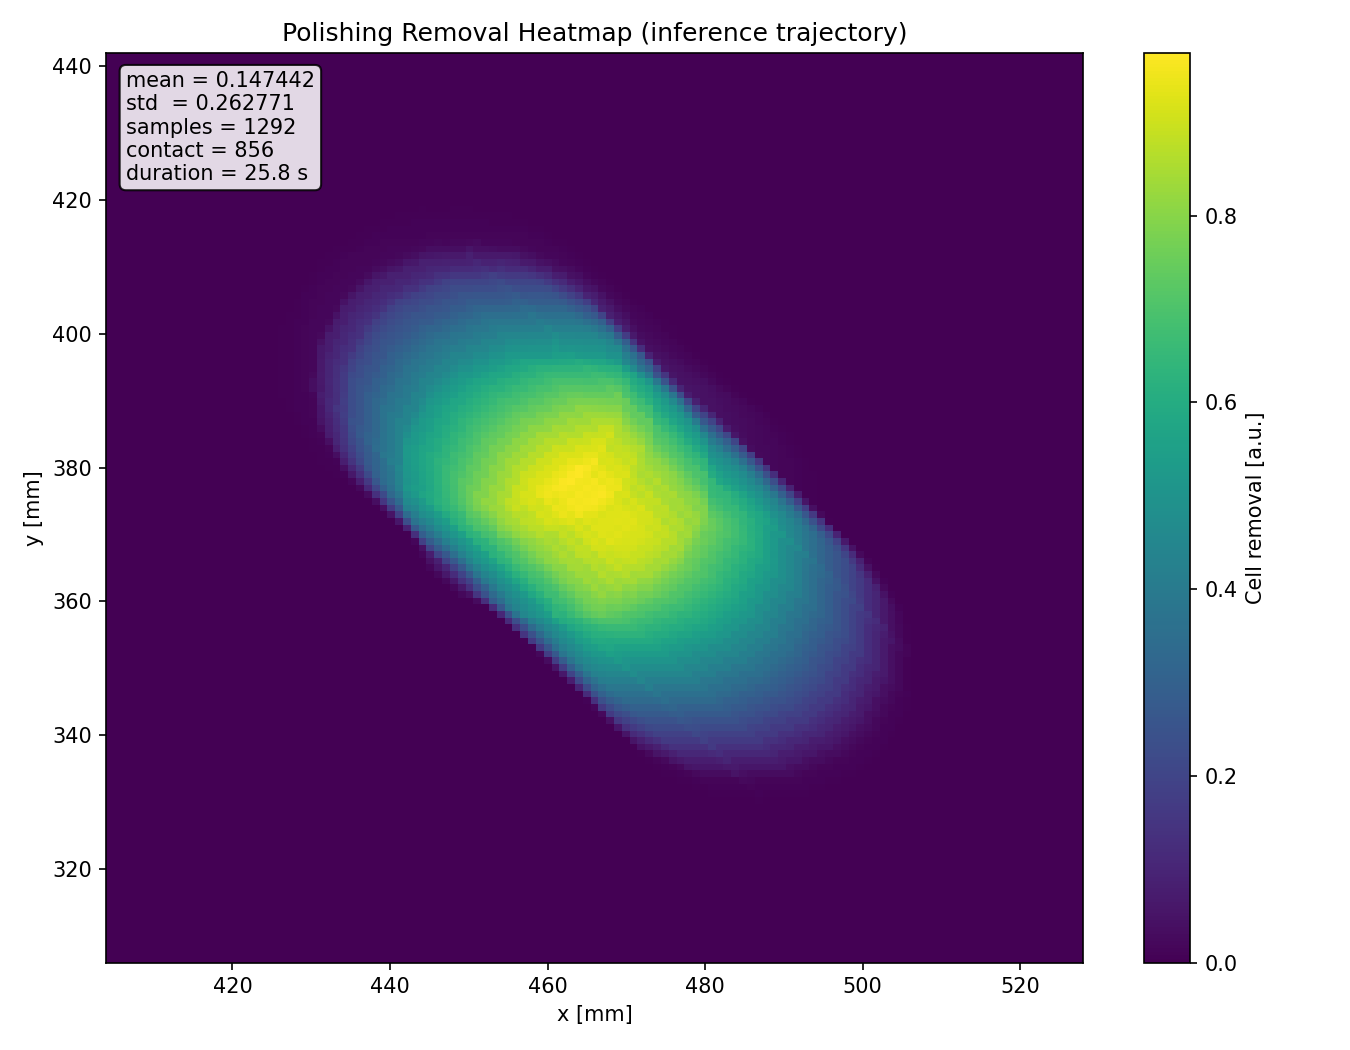
\includegraphics[width=\linewidth]{figures/E1_C1_diagnostic_heatmap.png}
\caption[Uncalibrated execution heatmap]{Historical execution-derived heatmap from E1 C1 on 14 October 2026, reproduced with its original axes and colorbar. Values are an uncalibrated model diagnostic in arbitrary units. They are not measured removal depth, effective contact footprint, or surface-quality improvement. This historical illustration is separate from the 15 October primary E1 cohort.}
\label{fig:diagnostic_heatmap}
\end{figure}

The implementation and generated artifact support calling this an implemented diagnostic extension. They do not support the older claim of a calibrated material-removal model. Its spatial distribution may help inspect where modeled processing exposure accumulated, but equal dose is not demonstrated equal removal on the actual specimen.

\section{Blending and Adaptive Execution Assets}
\label{chap:blending}
The project also contains finite local blending-path generation from an existing dose map, construction of an additional spatial target, and time allocation along a path. The 13 October extension prepares a sequence in which an initial skill is followed by a separate blending pass and diagnostic displays. Its archived validation includes offline planning from an earlier execution. That is evidence of an implemented extension, not an E1--E3 surface-uniformity result.

Separate 14 October adaptive-velocity records provide development experience with reference-clock progression and replanning. The located runtime files contain five online-OFF development attempts across multiple versions. Their completion status does not establish a controlled adaptive ON/OFF process-quality comparison. A later source revision addresses a recorded stalled reference-clock case, but its README explicitly distinguishes offline checking from a new physical run. These records are therefore kept outside the nominal E2 A/B/C cohort.

\begin{table}[tbp]\centering\small
\caption[Status of inherited extensions]{Status of inherited extensions relative to the main thesis evidence.}
\label{tab:extension_status}
\begin{tabularx}{\textwidth}{P{0.32\textwidth}X}
\toprule Asset & Supported status \\ \midrule
Execution heatmap & Implemented and generated from runs; uncalibrated arbitrary-unit diagnostic. \\
Finite blending planner & Implemented; archived offline planning and integration preparation. Surface-quality improvement not established by the main comparisons. \\
Adaptive reference-clock execution & Separate versioned development attempts and code; controlled ON/OFF outcome benefit not established. \\
High-level residual RL for curved-surface restoration & Planned extension; completed skill-level training and quality-grounded evaluation not established in the selected evidence. \\
\bottomrule
\end{tabularx}
\end{table}

An earlier thesis concept proposed residual adjustments to orientation and feed velocity based on residual removal demand. That concept remains a possible extension, with its old formulation retained in the preserved source. Existing low-level learned mass/damping control is a different asset and does not validate that proposed high-level policy. The core motion--force skill in this thesis does not require a removal estimator, blending planner, or residual RL stage to count as an executable system.

\section{Scope and Limitations}
E1/E2 assess the nominal local task; E3 extends the evidence to the reported planar placements and directions. Arbitrary shapes, curved surfaces, height changes, and reference-Z robustness remain outside those observations. The tested direction transfer includes an explicit observation/image adapter and XY inverse transformation. It is not an isolated test of policy equivariance or of force observation's causal contribution to spatial transfer. The inherited blending/RL assets retain their separate implementation or planned status.

There is one recorded training seed per learned condition, distinct from the repeated robot executions. Original E1 shuffles R/T/C within five blocks, whereas \(R^{*}\) is a separate-date one-then-four diagnostic. E2 runs A, then B, then C, using separate checkpoints; A/B also changes action dimension and force-target composition. Small cohorts and sample SDs establish neither statistical significance nor equivalence or population reliability. Setup, execution order, and operator timing remain possible contributors to the observed differences.

E3 is a selected development collection with retained retries and dates. N uses the existing HOME return, P1 uses PTP, and D1/D2 add commanded-release confirmation to PTP. These differences preclude treating duration or path length as a controlled removal-efficiency ranking. The image analysis is a post-hoc semiautomatic revision using stored photographs and saved visible-boundary annotations. D1's removal mean has \(n=4\); all five P2 final photographs and D1-4 are occluded. Hidden stain area is not estimated. The common 40/45/50 threshold sensitivity check describes segmentation dependence, not an uncertainty interval for future robot performance.

The thesis revision can reproduce the exact reported E3 integer-area calculation and the inherited E1/E2 precision aggregates. The original research repository, R* precision CSV/run identifiers, and E3 original image-pair/annotation files were not accessible on this PC. The supplied reports, unchanged embedded evidence panels, and explicit source-status manifest preserve the available evidence without claiming a fresh audit of those unavailable originals.

E1 automatic completion, E2 operator completion, and E3 image-area reduction remain distinct. A4's successful time is null; its \AfourInterval~s interruption and all-attempt force/path values remain. C5 stays in the original C group; C6 is additional. Metal depth, mass, roughness, and micro-scratch restoration are not independently measured, and an unrecorded controller-applied target still prevents force-tracking-error claims. These are limits of interpretation, not additional experiments required to complete this manuscript.

\chapter{Conclusions}
\label{chap:conclusions}

Local robotic polishing requires a strategy for movement, contact loading, and time within a selected region. Human region specification supplies the spatial task, but does not by itself determine that temporal strategy. This thesis has addressed the resulting skill-generation problem through paired motion--force teaching, observation-conditioned sequence learning, and a common robot execution interface.

Tool position is learned relative to a frozen stain center and paired with orientation and target force on a shared sequence. The direction-transfer adapter aligns live XY and the policy image with the teaching direction, then restores generated XY by inverse rotation and center addition. Z, tool orientation, and force keep their conventions. The evaluated Flow Matching policy uses RGB, Cartesian state, and three-axis force history, with explicit coordinate restoration, pose conditioning, plan connection, and existing contact regulation. E1/E2 disable direction alignment; E3 evaluates the registered planar transfer using the same C checkpoint and normalizer. The implementation separates upper-level skill generation, lower-level contact control, and completion recognition.

The first research question compares strategy providers for the fixed human-specified task. In the primary E1 cohort, rules, force-inclusive replay, and the conditioned policy each complete the required contact--loaded-pass--exit procedure in all five planned executions. Replay has a shorter mean completion time and smaller time dispersion than C, while C has greater mean excess-force exposure. The learned skill is therefore an executable strategy through the common robot interface, and rules and replay are also effective alternatives within this nominal task. C5 remains in the original C comparison and C6 is a separate diagnostic. The latest summary distinguishes additional \(R^{*}\) from original T/C. Processing retiming is associated with a \RstarTimeGain~s (\RstarTimePercent\%) shorter mean than original R while preserving +18 N and the common execution settings. This separate diagnostic uses a quintic peak-feed parameter and does not establish an IL advantage at matched measured speed.

The second research question compares the force-information configurations while retaining lower-level feedback. The force-observing motion--force policy C has a \BCSeconds~s (\BCPercent\%) shorter mean operator-based completion interval than force-masked B, with five completed attempts in each. Motion-only A completes four of five attempts; A4 does not progress to release and is interrupted. It remains in all-attempt force, travel, and elapsed-interval statistics, while A's successful-time mean uses four completions. Timing, phase progression, and force exposure differ across the configurations, without a monotonic improvement from A through B to C or an identified cause for the single interrupted transition.

The third research question evaluates spatial reuse through an image-based processing outcome. In \EthreeMainN{} selected N/P1/D1/D2 runs, \EthreeImageN{} pairs permit whole-stain evaluation. Mean \(\pm\) sample SD board-marker area reductions are \EthreeNRemoval\(\pm\)\EthreeNSD, \EthreePoneRemoval\(\pm\)\EthreePoneSD, \EthreeDoneRemoval\(\pm\)\EthreeDoneSD, and \EthreeDtwoRemoval\(\pm\)\EthreeDtwoSD\%, respectively. D1-4 remains selected with an unavailable removal value due to tool occlusion. P2's five executed, occluded runs remain in the 25-run archive outside the main removal comparison. The results support reuse of the same policy together with task registration and the direction adapter within the tested planar placements, without new teaching or retraining.

The demonstrated scope combines contact-skill execution, observed force-information differences, and E3 image-based ink-area reduction. The latter neither establishes E1/E2 removal quality nor independently measures metal surface restoration, roughness, or micro-scratch removal. It also does not establish arbitrary geometry or height robustness. Existing dose, blending, and adaptive-execution assets remain separate extensions with their documented status.

The thesis links a human-specified local region to paired motion and force teaching, center-relative representation, conditioned Flow generation, shared execution, and three evaluation axes. Fixed rules and replay are effective in the nominal task; force-information composition is associated with different execution behavior; and the same registered skill achieves high condition-mean image-area reduction in the tested placements. These complementary results answer the three research questions within the available evidence.

\clearpage
\bibliographystyle{IEEEtran}\bibliography{Bibliography/ThesisRef}
\appendix
\chapter{Coordinates, Signals, and Reproduction}
\label{chap:appendix}
\label{app:signals}

\section{Pose and Force Signal Definitions}
The position vector is expressed in millimeters and orientation as a rotation vector in radians. The matrix \(R=\operatorname{Exp}([\rho]_\times)\) maps a vector in the calibrated tool frame to the robot base when it represents \(R_{B\leftarrow E}\). \([\rho]_\times\) is the skew-symmetric matrix associated with \(\rho\). The saved dataset transformation subtracts only \((c_x,c_y)\). The optional inference transformation additionally rotates center-relative XY by \(R_2(\alpha)\), with inverse rotation followed by center addition on output (Section~\ref{sec:stain_relative_generalization}). Both retain Z, tool rotation vectors, and force channels. The evaluated E1/E2 settings use \(\alpha=0\).

Teaching force is a three-component post-publisher measurement. Its associated tool orientation supplies the base-axis rotation in Equation~\eqref{eq:normal_force_projection}. Robot wrench feedback is already base expressed. A torque reference-point transformation would require a moment arm, but no torque transfer is needed for the three-force-component base projection used here. The available analysis does not infer a calibrated compliant contact point from a TCP-center trajectory.

\begin{table}[tbp]\centering\small
\caption[Force signal definitions]{Force signal roles used throughout the thesis.}
\label{tab:force_roles}
\begin{tabularx}{\textwidth}{P{0.31\textwidth}X}
\toprule Signal & Interpretation \\ \midrule
Teaching intention & Operator's approximate loading intention; not a numeric command trace. \\
Teaching recorded force & Measured interaction after the published processing path; used to construct learning supervision. \\
Policy force action & Denormalized output of the generator before executor gating and slew. \\
Executor transmitted target & Command-side force after shared processing; tangential target channels disabled in these comparisons. \\
Controller-applied reference & Target after internal controller processing; synchronized trace unavailable. \\
Robot measured force & Processed base-frame feedback used by the common gate, policy adapter, and recorded analysis. \\
\bottomrule
\end{tabularx}
\end{table}

\section{Learning and Temporal Parameters}
The force-cleanup dataset contains 15,963 paired frames in 42 compact episodes. The optimization and validation sets contain 38 and four episodes. Validation episode identifiers are 35, 39, 22, and 37. Each epoch's training window construction uses 50 starts per episode, a 128-step target, and the archived phase-sampling weights. The partition stored in each normalizer matches the dataset manifest.

The force-history dimension is three, its sample count is 30, and the selected recurrent layer is a one-layer GRU with hidden size 64. The state encoder receives pose and current force together in B/C. A removes the force state dimensions and history encoder. B retains the history architecture with zeroed conditioning. Physical force remains available to common execution in all conditions.

The training horizon, reference stride, inference timer, command period, and logging cap describe different mechanisms:
\begin{table}[tbp]\centering\small
\caption[Distinct clocks and sampling settings]{Distinct clocks and sampling settings.}
\label{tab:clock_definitions}
\begin{tabularx}{\textwidth}{P{0.39\textwidth}X}
\toprule Mechanism & Value or meaning \\ \midrule
Teaching paired sample grid & Nominal 30 Hz; original receipt times retained in merged HDF5. \\
Action sequence & 128 samples, nominal 30 Hz. \\
Nominal new-plan stride & 120 action samples, approximately 4 s. \\
Inference callback timer & 5 Hz, subject to plan-age gating. \\
Flow integration & 10 dimensionless updates per generated chunk. \\
Command publication & Nominal 125 Hz (0.008 s). \\
E1 actual receipt-event recording & Approximately 125 Hz in the 15 October primary cohort; distinct subscription receipts. \\
E2 feedback CSV logging & 20 Hz cap; approximately 18 Hz observed in the 13 October archive. \\
Analysis support & Receipt-time ZOH force and within-support pose interpolation; maximum gap 0.2 s. \\
\bottomrule
\end{tabularx}
\end{table}

\section{Reproducing the Manuscript and Figures}
The revised project is independent of the original thesis outputs. Its build retains the original pdfLaTeX/KoTeX/BibTeX chain and copies the existing school style without editing it. The body retains equal top and bottom margins of 25 mm. The cover remains a draft because the source did not establish author, adviser, committee, or submission details.

From this revised project directory, the full manuscript and separate cover are built with
\begin{verbatim}
bash build.sh
\end{verbatim}
The figures and tables can be regenerated from the bundled extracted data without the robot repository:
\begin{verbatim}
python3 scripts/update_results_20261103.py
python3 scripts/export_information_diagram_20261103.py
bash build.sh
\end{verbatim}
The current regeneration entry point reads bundled E1/E2 precision CSVs and the unchanged report copies in \path{provenance/results_20261103/reports/}. It recalculates the E3 percentages from the report's integer pixel areas and uses the additional R report's authoritative summary. It performs no new segmentation, physical experiment, model loading, or evaluator audit. The earlier collection and plot scripts remain historical reproduction sources and are not the current result-update entry points. Source availability and precision are explicit in \path{results_manifest_20261103.csv} and \path{provenance/results_20261103/metric_definitions.json}.

The figure manifest records original files, run identifiers, frame indices or video offsets, transformations, and manuscript locations. Conceptual diagrams reside in the chapter LaTeX and are distinguished from measured plots in their captions. No generated photograph is used.

\chapter{Experiment Versions and Provenance}
\label{app:provenance}

\section{Selected Models and Dataset}
The dataset and models are the force-cleanup revision dated 12 October, with training completed on 13 October 2026. All three selected checkpoints have their own normalizer. The best epochs are 39, 42, and 42, while final epoch is 499. The stored checkpoint selection rule is minimum validation loss over 500 epochs. The inherited model manifest records the earlier CPU metadata inspection. This revision retains that evidence without loading checkpoints or retraining.

\begin{table}[tbp]\centering\small
\caption[Selected model identifiers]{Short SHA-256 identifiers of the selected checkpoints and normalizers. Complete values are included in the supplied model manifest.}
\label{tab:model_provenance}
\begin{tabular}{lll}
\toprule Model & Checkpoint prefix & Normalizer prefix \\ \midrule
A & \texttt{2ea204ab65fb} & \texttt{ae7d07adf65a} \\
B & \texttt{080103e6c2ed} & \texttt{d7c917b8246c} \\
C & \texttt{60d55e7092cb} & \texttt{09111fa4acc3} \\
\bottomrule
\end{tabular}
\end{table}

The compact replay episode is linked to the source merged HDF5 recorded at 16:18 on 19 August 2026, source episode \texttt{ep\_0003}. Its compact action and observation pose/force arrays contain 443 frames. The original source-time array is retained for T rather than replaced by an assumed constant period. The exact source paths and extraction fields are recorded in the supplied episode metadata.

\section{Primary E1 Version and Membership}
The physically executed primary cohort is
\begin{quote}\small\path{E1_CT_pass_height_v2_nominal_dev_20261015}\end{quote}
with configuration \texttt{e1ct\_46de718a23a2a7cf}, evaluator \texttt{pass\_height\_ref\_v2}, and observer \texttt{received\_observations\_v2}. The source report freezes the 15 planned run identifiers. Each planned slot has one started primary execution, and the original C5 remains the run ending in \texttt{230120\_b45d2f021b}. Its full identifier and the additional C6 identifier are recorded in the cohort manifest.

C6 is the later execution ending in \texttt{233551\_9021584d0a}. It retains repeat index 5 and the source retry link in the original archive, but is displayed as C6 for diagnostic interpretation. The subsequent session list therefore has 16 entries, while the primary E1 set remains the report-frozen 15. The explicit selection uses planned slots and original identifiers rather than the most recent record per repeated index. The same C checkpoint and frozen execution setting are retained.

The handoff \path{baseline_manifest.json} still contains preparation-era zero-attempt fields. The actual report, original execution evidence, and frozen report membership supersede those status fields for this thesis. The nominal placement is operator reported; the configured approximate surface Z is not a per-trial physical measurement. LOW/HIGH and reference-offset robustness are outside the completed evaluation scope.

\section{Historical E1 Development and Height-Only Replay}
\label{app:e1_history}
The 14 October development session, \texttt{E1\_CT\_sync\_confirm\_dev\_20261014}, uses configuration \texttt{e1ct\_61a19f7d7337a82c} and the initial-contact height reference. Its started order is R, then T, then C. All 15 started runs show the required loaded pass, while the old exit criterion reports R 3/5, T 4/5, and C 5/5. Table~\ref{tab:e1_historical_primary} preserves this historical comparison separately from the primary 15 October results.

\begin{table}[tbp]\centering\footnotesize
\caption[Historical 14 October E1 results]{Historical 14 October E1 development cohort with the initial-contact height reference. Completed-time means use \(n=3,4,5\) for R/T/C; excess-force summaries retain five started runs per method. These executions are not pooled with the primary cohort.}
\label{tab:e1_historical_primary}\begin{tabular}{lcrr}
\toprule
Method & Completed/started & Completed time (s) & $J_{\mathrm{excess}}$ (N\,s) \\
\midrule
R & 3/5 & $29.58 \pm 0.03$ & $0.000 \pm 0.000$ \\
T & 4/5 & $12.86 \pm 0.01$ & $0.005 \pm 0.011$ \\
C & 5/5 & $15.67 \pm 3.60$ & $2.323 \pm 2.493$ \\
\bottomrule
\end{tabular}

\end{table}

The old release requirement was
\begin{equation}
 Z(t)\geq z_{\mathrm{contact}}+5\ \mathrm{mm},
 \label{eq:original_release}
\end{equation}
with OFF and rise sustained together for 0.2 s. R1, R3, and T4 were sensitive to the early height reference. The archived height-only replay changes that reference for the same observations and reports 5/5 for every method (Table~\ref{tab:e1_replay}). It supplies no new physical executions and does not reconstruct the later receipt-event observer.

\begin{table}[tbp]\centering\small
\caption[Historical E1 height-only replay]{Height-only offline replay of the 14 October records. This secondary sensitivity analysis changes the release reference, retains the recorded trajectories, and adds no independent trials.}
\label{tab:e1_replay}\begin{tabular}{lcr}
\toprule
Method & Replay completed & Replay time (s) \\
\midrule
R & 5/5 & $27.24 \pm 1.28$ \\
T & 5/5 & $12.84 \pm 0.02$ \\
C & 5/5 & $15.64 \pm 3.59$ \\
\bottomrule
\end{tabular}

\end{table}

\figfull{e1_height_reference.pdf}{Historical 14 October release thresholds using the initial-contact and successful-pass references. Both are derived from the same stored TCP traces. This diagnostic is distinct from the physically executed 15 October primary evaluator.}{fig:e1_height_reference}

An original 14 October R5 registration did not reach execution start and was followed by a started retry. Its source identifiers remain in the historical provenance. This bookkeeping does not apply to the 15 October primary cohort, whose original 15 slots contain no non-start or retry. Earlier prepared but unexecuted sessions are historical preparation records and are not incomplete requirements of the present thesis.

\section{E2 Versions and the A4 Correction}
The selected E2 cohort uses the force-cleanup revision of 13 October. Each actual \texttt{runtime.json} names its model revision, observation settings, and common executor. The run inventory orders the attempts A1--A5, B1--B5, and C1--C5. Preparation-only runtime files are not used as substitutes for these actual run files.

The old E2 report applied a common operator-confirmed completion interpretation to all 15 attempts. The later task instruction specifically corrects A4. This thesis adopts that field correction and stores it in \path{data/e2_operator_correction.json}. The original software event remains \texttt{operator\_finish}, followed by the original normal-completion stop-path event. The derived task outcome is separately marked incomplete contact release. The original elapsed time 28.750087346 s remains the interruption interval.

The correction changes only the successful-time aggregation and task interpretation. A4 remains in all five-attempt statistics for force, travel, and elapsed interval. No surface image, raw force sample, event timestamp, or checkpoint is edited. The corrected table can be reconstructed from \path{data/e2_runs_corrected.csv}.

\section{Sources for Implemented Extensions}
The execution heatmap is generated by the existing polishing-removal recorder. The finite blending path and dose tools are in the local blending module and the 13 October extension package. The adaptive-velocity development records are versioned separately under the 14 October results directory. Their runtime metadata identifies them as adaptive-execution development rather than the primary E2 force ablation.

\chapter{Individual Outcomes and Evidence Boundaries}
\label{app:runs}

\section{E1 Primary Executions}
Table~\ref{tab:e1_all} lists all original primary E1 executions on 15 October. Every row completes the specified contact--pass--exit procedure, including C5. The recorded order identifies the shuffled blocks. C6 is reported separately in Table~\ref{tab:e1_c5_c6} and is not a sixth observation in any primary C mean.

\begin{table}[tbp]\centering\small
\caption[Individual primary E1 outcomes]{All 15 primary E1 executions under \texttt{pass\_height\_ref\_v2}. All are procedurally completed. Full run identifiers, original labels, and source paths are preserved in the cohort manifest.}
\label{tab:e1_all}\begin{tabular}{lcrrr}
\toprule
Run & Order & \makecell{Completion\\(s)} & \makecell{$J_{\mathrm{excess}}$\\(N\,s)} & \makecell{Peak $F_z^B$\\(N)} \\
\midrule
R1 & 2 & 29.424 & 0.000 & 22.81 \\
R2 & 5 & 29.516 & 0.000 & 23.18 \\
R3 & 7 & 29.546 & 0.000 & 22.90 \\
R4 & 10 & 29.573 & 0.000 & 22.52 \\
R5 & 13 & 29.625 & 0.000 & 22.02 \\
T1 & 1 & 12.828 & 0.037 & 32.85 \\
T2 & 4 & 12.908 & 0.001 & 30.96 \\
T3 & 9 & 12.896 & 0.580 & 38.24 \\
T4 & 11 & 12.920 & 0.010 & 31.91 \\
T5 & 15 & 12.931 & 0.000 & 30.43 \\
C1 & 3 & 11.694 & 0.048 & 32.89 \\
C2 & 6 & 12.876 & 0.431 & 34.35 \\
C3 & 8 & 12.740 & 0.237 & 33.43 \\
C4 & 12 & 11.766 & 0.068 & 32.65 \\
C5 & 14 & 18.024 & 6.413 & 40.21 \\
\bottomrule
\end{tabular}

\end{table}

\section{E2 All Attempts}
Table~\ref{tab:e2_all} distinguishes successful completion intervals from time to interruption. All original stop requests are retained. In particular, the missing A4 completion time is not a missing raw record.

\begin{table}[tbp]\centering\small
\caption[Individual E2 corrected task outcomes]{Individual E2 task outcomes after the A4 field correction. ``Operator completed'' uses the recorded operator interpretation; it is not an automatic E1 evaluation.}
\label{tab:e2_all}\begin{tabular}{llrr}
\toprule
Run & Task outcome & Completion (s) & Interval to stop (s) \\
\midrule
A1 & operator completed & 16.787 & 16.787 \\
A2 & operator completed & 16.445 & 16.445 \\
A3 & operator completed & 18.581 & 18.581 \\
A4 & interrupted & \NA & 28.750 \\
A5 & operator completed & 18.777 & 18.777 \\
B1 & operator completed & 18.690 & 18.690 \\
B2 & operator completed & 18.511 & 18.511 \\
B3 & operator completed & 19.508 & 19.508 \\
B4 & operator completed & 18.693 & 18.693 \\
B5 & operator completed & 18.671 & 18.671 \\
C1 & operator completed & 15.902 & 15.902 \\
C2 & operator completed & 15.297 & 15.297 \\
C3 & operator completed & 15.597 & 15.597 \\
C4 & operator completed & 16.751 & 16.751 \\
C5 & operator completed & 15.618 & 15.618 \\
\bottomrule
\end{tabular}

\end{table}

The archived video inventory contains B/C videos but no A videos. The illustrated C1 WebM has an incomplete container ending; only decodable frames are used. It is not treated as a continuous independent proof of full task completion. Snapshot timing and varying tool viewpoint also limit before/after interpretation.

\section{Cohort Membership and Interpretation}
The original \path{data/cohort_manifest.csv} and JSON counterpart remain historical records of the original E1 15, E2 15, and diagnostic C6. The current \path{results_manifest_20261103.csv} adds the separate five \(R^{*}\) entries and all 25 E3 entries. E3 retains the report's original run identifiers, main/archive role, image availability, and occlusion reason. The additional R report does not print its original run identifiers; those fields remain empty, explicitly marked unavailable, rather than inferred from display labels.

The precision summary, prose macros, and regenerated result plots use \path{data/results_summary_20261103.json}. E1/E2 execution cohorts, original R and \(R^{*}\), and image versus procedure outcomes remain separate. Earlier analysis checks are retained as earlier checks; they are not relabeled as newly performed source validation.

\section{Original E1 Strategy Traces and Additional Cases}
\label{app:execution_cases}
The original 15 October R/T/C summary is preserved here separately from the latest R*/T/C table. Each method has five completed executions. The following traces retain original C5 and exclude C6 from group statistics.

\begin{table}[tbp]\centering\footnotesize
\caption[Original 15 October E1 comparison]{Original R/T/C comparison on 15 October 2026; mean \(\pm\) sample SD, \(n=5\). This table preserves the original cohort and is not pooled with additional \(R^{*}\).}
\label{tab:e1_original_comparison}\begin{tabular}{lcrr}
\toprule
Method & Completed/started & Time (s) & $J_{\mathrm{excess}}$ (N\,s) \\
\midrule
R & 5/5 & $29.537 \pm 0.075$ & $0.000 \pm 0.000$ \\
T & 5/5 & $12.897 \pm 0.041$ & $0.125 \pm 0.254$ \\
C & 5/5 & $13.420 \pm 2.630$ & $1.440 \pm 2.785$ \\
\bottomrule
\end{tabular}

\end{table}

\figfull{e1_force_all.pdf}{Actual received robot-base \(F_z\) for all 15 original E1 runs, from execution start to first completion. Values use the archived ZOH display. The dashed teaching Q95 is an empirical analysis reference. C5 remains included.}{fig:e1_force_all}
\figfull{e1_xy_all.pdf}{All 15 original E1 TCP-center XY paths through first completion. The shaded region is the fixed 25 mm evaluation band, not a contact footprint or removal map.}{fig:e1_xy_all}

\subsection{Original C5 and Additional Diagnostic C6}
The original primary C5 completes at \CfiveTime~s, with \(J_{\mathrm{excess}}=\CfiveExcess\) N\,s and observed peak \CfivePeak~N. Its required loaded pass completes at \CfivePass~s. These values remain in every primary C summary. The additional execution at 23:35 on the same date is displayed as C6. Its source retains repeat index 5 and a retry link to C5; those original fields are preserved in the manifest, while the analysis treats it as an additional post-comparison diagnostic rather than replacing the planned slot.

\begin{table}[tbp]\centering\footnotesize
\caption[Original C5 and additional diagnostic C6]{Individual E1 executions with the same recorded evaluator. C5 belongs to the original primary five; C6 is additional diagnostic evidence. Times are relative to each execution start. Single-run values are shown without mean or SD.}
\label{tab:e1_c5_c6}\begin{tabular}{lrr}
\toprule
Metric & Original C5 (primary) & C6 (diagnostic) \\
\midrule
Completion time (s) & 18.024 & 11.728 \\
First confirmed contact (s) & 4.464 & 4.420 \\
Required pass complete (s) & 16.488 & 10.980 \\
Working reference Z (mm) & 174.209 & 174.411 \\
Required exit Z (mm) & 179.209 & 179.411 \\
Observed peak force (N) & 40.211 & 35.006 \\
$J_{\mathrm{excess}}$ (N\,s) & 6.413 & 0.471 \\
Time above reference (s) & 1.829 & 0.260 \\
Recorded contact losses & 1 & 0 \\
\bottomrule
\end{tabular}

\end{table}

C6 completes at \CsixTime~s, with \(J_{\mathrm{excess}}=\CsixExcess\) N\,s and peak \CsixPeak~N. The original outcome file and actual receipt events support these quantities. Figure~\ref{fig:e1_c5_c6} shows that C5's first successful pass occurs later, while initial contact confirmation occurs at a similar elapsed time. C5 records one contact loss and C6 none. These stage observations describe the traces and do not establish a failure mechanism.

\figfull{e1_c5_c6.pdf}{Separate traces for original C5 and additional C6. Top: received force with teaching Q95 dashed. Bottom: measured Z with required exit height dashed. Vertical dotted gray, dashed blue, and solid orange lines mark confirmed contact, required-pass completion, and first procedural completion. Full analysis windows are shown with a common time axis. C6 is not included in the primary mean.}{fig:e1_c5_c6}

C5's longer execution and larger excess integral are not reproduced in C6. One additional execution does not show that the variability is resolved, that C5 was erroneous, or that the model improved. The original five-run comparison remains the basis for R/T/C conclusions.


\section{E2 Force Traces and Transition Cases}
\figfull{e2_force_all.pdf}{All measured E2 base-force traces from execution start to first operator stop request. A4 remains in A's five curves. Each curve uses native recorded values with ZOH; the plots do not infer a controller-applied force target.}{fig:e2_force_all}
\subsection{Phase Transitions and Execution Cases}
A4 is a direct counterexample to treating every normal-completion software event as task success. The operator reports that the tool remained in contact rather than progressing to release, and interrupted the attempt after \AfourInterval~s. Its measured mean \(F_z^B\) is \AfourMeanForce~N and its interval with recorded force at or above 3 N is \AfourContactTime~s. The trace is consistent with prolonged loading. The field report establishes the task interpretation; the trace does not independently establish why the transition failed.

\figfull{e2_transition_cases.pdf}{Two retained E2 transition cases. A4 is included because of the operator-confirmed release-transition failure. B4 is included because it has the maximum recorded contact-gate transition count, 38. Full force and Z traces are shown. Rapid gate transitions are a software contact diagnostic, not an independently counted number of physical impacts.}{fig:e2_transition_cases}

B4 illustrates a different phenomenon: the common instantaneous gate toggles repeatedly near contact transitions, with 38 recorded changes. The group mean gate-transition counts are 2.6\(\pm\)0.9 for A, 12.4\(\pm\)14.8 for B, and 3.6\(\pm\)1.7 for C. B's dispersion is strongly influenced by B4; it is retained. Threshold crossings, baseline behavior, and transition timing can all affect these counts. They are not sufficient to diagnose an encoder failure or a physical contact-instability mechanism.

E2 C shows a relatively compact range of operator-based intervals and XY travel, but B's completed-time SD is smaller. Repeatability therefore depends on the quantity being considered. A leave-one-out deviation from other executions, where used in earlier diagnostics, would measure between-run repeatability rather than agreement with the teaching or controller force-tracking accuracy. The present primary comparisons use the explicitly reported timing, force, and travel quantities.

\section{E1/E2 Qualitative Image Evidence}
Figure~\ref{fig:e1_photos} shows the first started run of each E1 method, selected by run index without screening for the best image or result. The provider's initial and final snapshots have different viewpoints and times as the tool moves. They can illustrate the marked task and visible appearance but cannot quantify common-area removal. All-trial numerical results accompany these examples.

\figfull{e1_snapshot_panel.pdf}{Actual provider snapshots from the original E1 R1, T1, and C1 executions on 15 October 2026. Initial/final denote saved provider snapshots rather than matched metrology exposures; viewpoint, occlusion, and timing can differ. Visible marking changes do not measure scratch depth or surface restoration.}{fig:e1_photos}

\figfull{e2_sequence.pdf}{Uniformly spaced camera-pane crops from the decodable portion of the first E2 C video. Only the adjacent diagnostic panel is omitted; camera overlays are retained. Times are video offsets, not synchronized stage-event times. The archived WebM ends prematurely and is not used to certify a complete exit sequence. A4 has no archived video.}{fig:e2_sequence}

The existing heatmaps are execution-derived model diagnostics in arbitrary units. Their values are not measured removal depth, roughness reduction, or scratch-removal percentage. They are therefore outside the primary success criterion. A visually diminished marking and a completed contact procedure can be useful observations without supporting a stronger claim about metal surface quality.


\chapter{Additional R Diagnostic and E3 Image Archive}
\label{app:e3_archive}

\section{Additional R Executions and Source Precision}
\begin{table}[tbp]\centering\footnotesize
\caption[Additional R diagnostic runs]{All five \(R^{*}\) executions on 19 October, at the report's printed per-run precision. The first diagnostic precedes four extension runs. These do not replace the original R1--R5. Time is first automatic procedure completion; pass speed uses the successful loaded-pass support.}
\label{tab:e1_rstar_all}\begin{tabular}{lrrrr}
\toprule
Run & Time (s) & $J_{\mathrm{excess}}$ (N\,s) & Peak (N) & Pass (mm/s) \\
\midrule
R$^{*}$1 & 22.481 & 0.000 & 21.488 & 10.696 \\
R$^{*}$2 & 25.319 & 0.000 & 22.000 & 10.887 \\
R$^{*}$3 & 25.520 & 0.000 & 20.541 & 10.886 \\
R$^{*}$4 & 25.458 & 0.000 & 22.727 & 10.822 \\
R$^{*}$5 & 25.420 & 0.000 & 20.944 & 10.915 \\
\bottomrule
\end{tabular}

\end{table}

The source is the 17-page additional-R report, pp.1--5 and 17. It records separate configuration identifiers for the first diagnostic and four extension runs, preserved in \path{data/e1_rstar_report_runs.csv}, with the same frozen template, feed, runtime source, +18 N target, and v2 evaluator/observer. The separate configuration/session identifiers document the one-then-four history. The original input manifest, template file/hash, and full per-run CSV/run identifiers could not be reopened in this revision environment; agreement beyond the report's printed precision is not asserted.

Reaggregation of the printed times gives 24.8396 s and sample SD 1.320516 s, agreeing on rounding with the report's authoritative \EoneRstarTime\(\pm\)\EoneRstarTimeSD~s. The current summary retains that published precision rather than implying recovery of the original unrounded values. All five zero excess integrals and the unusually short first run remain included.

\section{E3 Main-Run Pixel Areas}
\begin{table}[tbp]\centering\footnotesize
\caption[Individual E3 main-run image areas]{All 20 main selected N/P1/D1/D2 runs. Areas are exact integer pixel counts printed on pp.5--9 of the 39-page report; percentages are recomputed using Equation~\eqref{eq:e3_removal}. D1-4's final area and percentage remain null. Image evaluability is not procedure success.}
\label{tab:e3_all_runs}\begin{tabular}{lrrrl}
\toprule
Run & $A_{\mathrm{before}}$ (px) & $A_{\mathrm{after}}$ (px) & Removal (\%) & Note \\
\midrule
N-1 & 837 & 0 & 100.000 & image evaluable \\
N-2 & 879 & 0 & 100.000 & image evaluable \\
N-3 & 699 & 0 & 100.000 & image evaluable \\
N-4 & 697 & 0 & 100.000 & image evaluable \\
N-5 & 712 & 0 & 100.000 & image evaluable \\
P1-1 & 858 & 31 & 96.387 & image evaluable \\
P1-2 & 846 & 6 & 99.291 & image evaluable \\
P1-3 & 772 & 11 & 98.575 & image evaluable \\
P1-4 & 846 & 2 & 99.764 & image evaluable \\
P1-5 & 799 & 50 & 93.742 & image evaluable \\
D1-1 & 546 & 41 & 92.491 & image evaluable \\
D1-2 & 676 & 0 & 100.000 & image evaluable \\
D1-3 & 680 & 0 & 100.000 & image evaluable \\
D1-4 & 700 & \NA & \NA & tool occlusion \\
D1-5 & 798 & 0 & 100.000 & image evaluable \\
D2-1 & 768 & 79 & 89.714 & image evaluable \\
D2-2 & 738 & 13 & 98.238 & image evaluable \\
D2-3 & 794 & 128 & 83.879 & image evaluable \\
D2-4 & 743 & 13 & 98.250 & image evaluable \\
D2-5 & 684 & 12 & 98.246 & image evaluable \\
\bottomrule
\end{tabular}

\end{table}

The report's per-run identities and areas are captured in \path{data/e3_report_area_runs.csv}. The exact per-run ratios reproduce the reported main condition means and sample SDs. P1 ranges from 93.742 to 99.764\%, evaluable D1 from 92.491 to 100.000\%, and D2 from 83.879 to 98.250\%. The eight 100\% observations (five N and D1-2/3/5) mean black-ink nondetection under the established criterion.

\section{Occlusion, Interruption, and P2 Exclusion}
\begin{table}[tbp]\centering\footnotesize
\caption[Executed P2 archive records]{P2 was executed five times and remains in the original 25-run selection. Every final photograph is tool-occluded. The initial areas are retained; whole-stain final areas and removal percentages are unavailable, not zero. P2 is outside the main four-condition removal evaluation.}
\label{tab:e3_p2_archive}\begin{tabular}{lrrl}
\toprule
Run & $A_{\mathrm{before}}$ (px) & Image result & Original stop \\
\midrule
P2-1 & 777 & unavailable & \texttt{operator\_finish} \\
P2-2 & 773 & unavailable & \texttt{operator\_finish} \\
P2-3 & 652 & unavailable & \texttt{operator\_finish} \\
P2-4 & 717 & unavailable & \texttt{operator\_finish} \\
P2-5 & 778 & unavailable & \texttt{operator\_finish} \\
\bottomrule
\end{tabular}

\end{table}

D1-4 retains \texttt{manual\_abort}; its interruption-time diagnostic frame contains visible residual marking and final tool occlusion. The report identifies the frame as received 34.5 ms before the abort request (source stamp approximately 0.55 s before it). No post-HOME photograph is available. The visible region is not used to estimate hidden total residual area. P2's initial frames are same-run pre-execution raw RGB, replacing initially occluded photographs; the final occlusion remains. These records are not removed or renamed in the archive.

\begin{figure}[tbp]\centering
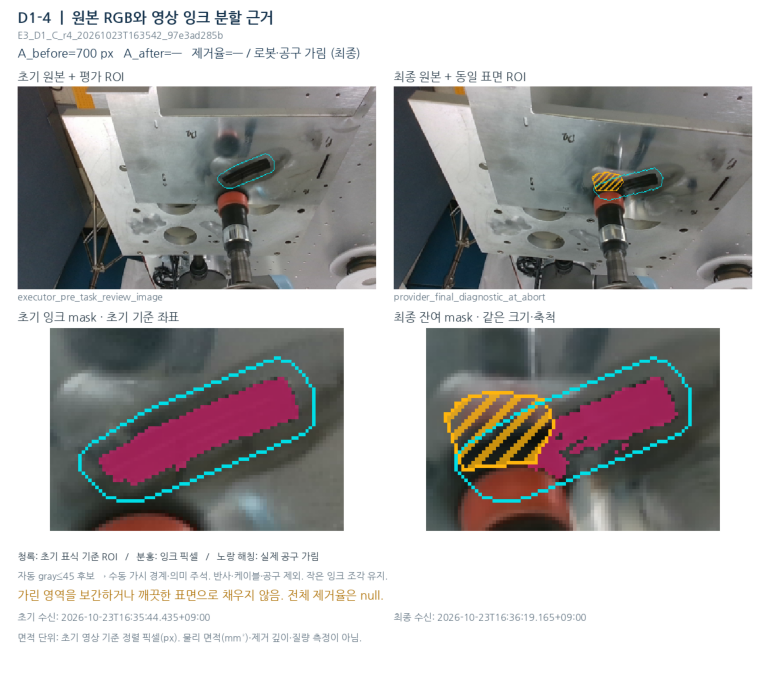
\includegraphics[width=.88\linewidth]{figures/e3_D1-4_report_evidence.png}
\caption[D1-4 retained interruption and occlusion evidence]{Unchanged report-embedded D1-4 evidence, from p.28. Cyan marks the common ROI, magenta denotes annotated visible ink, and hatching indicates tool occlusion. The visible residual and original interruption are preserved; the whole-stain final area is unavailable. This is a report reproduction, not a newly registered or resegmented image pair.}
\label{fig:e3_d1_occlusion}
\end{figure}

\begin{figure}[tbp]\centering
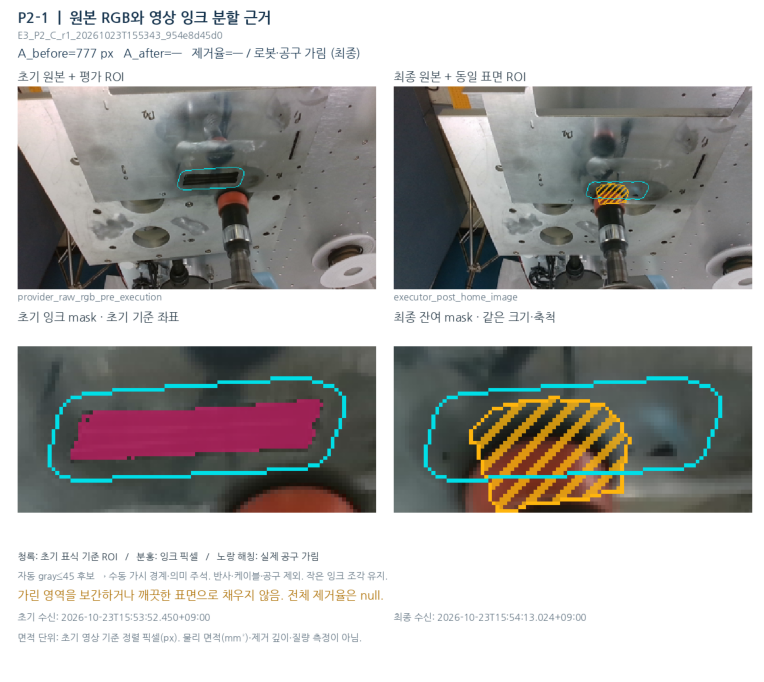
\includegraphics[width=.88\linewidth]{figures/e3_P2-1_report_evidence.png}
\caption[P2 retained final occlusion example]{Unchanged P2-1 report evidence, p.20. Its pre-execution replacement initial image exposes the stain, while final tool occlusion prevents whole-stain removal measurement. All five P2 panels are retained in the supplied evidence archive; P2 is not an unexecuted condition.}
\label{fig:e3_p2_occlusion}
\end{figure}

\section{Reused Segmentation Sensitivity and Procedure Diagnostics}
The report's sensitivity check keeps annotations and ROI fixed and changes the gray threshold equally in before/after images. The published condition means are reproduced below at their printed precision; no new threshold or manual boundary is selected.

\begin{table}[tbp]\centering\small
\caption[Archived E3 threshold sensitivity]{Existing sensitivity results from the image report, p.36. Values are condition-mean percentages; main gray threshold is 45. These are not sample SD or confidence intervals. D1 uses four images throughout.}
\label{tab:e3_sensitivity}
\begin{tabular}{lrrr}\toprule
Condition & gray \(\leq40\) & gray \(\leq45\) & gray \(\leq50\) \\ \midrule
N & 100.000 & 100.000 & 100.000 \\
P1 & 97.912 & 97.552 & 96.914 \\
D1 & 98.124 & 98.123 & 98.056 \\
D2 & 94.659 & 93.665 & 92.932 \\
\bottomrule\end{tabular}
\end{table}

The old v2 procedure outcomes, reproduced on p.37 of the image report, are 8 completed and 17 \texttt{observation\_unavailable} in the original 25-run selection, with 24/25 HOME returns. These are auxiliary diagnostic labels on that archive, not removal successes or outcomes for the main 20-run subset. Image inclusion is independent of them. The original execution report and its full force/path CSV were not present locally; this revision cites the preserved image-report diagnostic summary without claiming a new calculation.

\section{Evidence Availability and Reproduction}
The 39-page report's pp.10--34 contain one before/after RGB, ROI, mask, and occlusion evidence panel per selected run. All 25 embedded panels are losslessly extracted to \path{provenance/results_20261103/e3_report_panels/}. The panel manifest maps each to its original run identifier and report page. The main figure uses repeat 1 of each main condition, with fixed identical crop rectangles documented by the regeneration script. These are display operations on existing report images and are never input to area measurement.

The report describes \path{image_pair_manifest.json} and its CSV counterpart, \path{analysis_config.json}, \path{annotations.json}, \path{occluded_runs.csv}, and the per-run raw RGB/ROI/mask files in the research repository. Those originals were not accessible on this PC. Thus this revision recovers exact printed integer-area statistics and unchanged photographic evidence at report level, while original file-path/hash and annotation reproduction remain document-source checks that cannot be claimed complete. The supplied four original PDF reports are preserved byte for byte. Registered E3 offsets and common-checkpoint/termination details additionally follow the user's confirmed revision record and are identified as such in the source map.


\chapter*{국문요약}
\addcontentsline{toc}{chapter}{국문요약}
\begin{center}\large\bfseries\thesistitlekr\end{center}

표면 마무리 공정에서 부품 전체의 균일 처리와 지정된 영역 주변의 국소 재작업은 서로 다른 요구를 가진다. 국소 폴리싱에서는 대상 영역에 맞추어 공구 이동, 접촉 힘, 작업 시간을 함께 구성해야 한다. 본 연구는 현재 장비로 미세 스크래치를 자율 판별하는 대신 사람이 처리 영역을 지정하는 설정을 사용한다. 공간 지시 이후에도 남는 동작·힘·시간 구성 문제에 대해, 규칙 기반 전략과 교시 재생에 비해 관측 조건부 학습이 어떤 수행 가치를 추가하는지 검토한다.

추적 기반 교시 장치로 공구 위치·자세, 3축 힘, RGB 영상을 시간적으로 대응하여 기록한다. 얼룩 중심 상대위치를 학습하고 얼룩 방향을 학습 기준에 정렬한다. Flow Matching 정책은 영상, 로봇 상태, 측정 힘 이력으로 위치·자세·목표 힘 시퀀스를 생성한다. 공통 실행 계층은 좌표 복원, 계획 연결, 명령 후처리를 수행하고 기존 하위 힘제어기가 접촉을 조절한다. 스킬 생성, 접촉 제어, 절차 완료 판정의 역할을 분리한다.

세 실험은 전략별 실행, 힘 정보 구성, 공간 재사용을 평가한다. E1에서 원 규칙 R, 힘 포함 교시 재생 T, 힘 조건부 정책 C는 각 5회에서 접촉--연속 부하 통과--이탈 절차를 완료했다. 최신 요약은 10월 19일의 추가 규칙 재실험 \(R^{*}\) 5회와 10월 15일 원 T/C를 구분하며, 원 R도 별도로 보존한다. \(R^{*}\)/T/C의 평균 완료시간은 각각 \EoneRstarTime, \EoneTTime, \EoneCTime{}초였다. T는 C보다 시간 분산과 초과 힘 적분이 작았다. \(R^{*}\)는 원 R보다 평균시간이 \RstarTimePercent\% 짧았으나, 이는 별도 추가 진단이며 실측 평균속도 정합 비교가 아니다. E2는 동작 전용 A와 힘 관측 유무에 따른 동작--힘 학습 B/C를 비교한다. A는 4/5회 완료했고, A4는 접촉 해제로 진행하지 못해 \AfourInterval{}초에 작업자가 중단했다. B/C는 각 5회 완료했으며 C의 평균 작업자 기준 완료시간은 B보다 \BCSeconds{}초(\BCPercent\%) 짧았다. 이는 E1의 자동 절차 완료시간과 다른 시간 정의다.

E3는 동일 C 체크포인트와 정규화기를 재교시·재학습 없이 다른 평면 위치·방향의 등록 작업영역에 적용한 학습 스킬의 위치·방향 전이 평가다. 저장된 전후 사진의 보드마카 잉크 면적 감소율을 공통 흑색 임계값과 보존된 가시 경계 수동 주석으로 평가했다. 본문 N/P1/D1/D2는 총 \EthreeMainN{}회이며 영상 평가 가능 시행은 \EthreeImageN{}회다. 조건별 제거율 평균\(\pm\)표본 SD는 각각 \EthreeNRemoval\(\pm\)\EthreeNSD, \EthreePoneRemoval\(\pm\)\EthreePoneSD, \EthreeDoneRemoval\(\pm\)\EthreeDoneSD, \EthreeDtwoRemoval\(\pm\)\EthreeDtwoSD\%이며 영상 유효 \(n=5,5,4,5\)다. D1-4는 D1의 5회에 남기되 최종 공구 가림으로 제거율만 산출하지 않았다. P2도 실행된 5회이며 모두 최종 가림으로 본문 주 평가에서 제외하고 원 25회 기록에 보존한다. 100\%는 해당 영상·분할 기준에서 잔여 흑색 잉크가 검출되지 않았다는 뜻이다.

결과는 인간 지정 국소 작업에서 학습 스킬의 실행 가능성, 힘 정보 구성별 실행 특성, 시험 배치 안에서 동일 정책과 작업 등록·방향 어댑터의 재사용을 뒷받침한다. 고정 작업에서는 규칙과 교시 재생도 유효했다. E3의 영상 면적 감소는 E1/E2의 제거 품질을 소급 검증하지 않으며, 금속 제거 깊이·질량·거칠기·미세 스크래치 복원은 독립 계측하지 않았다.

\vspace{0.4cm}
\noindent\textbf{주요어:} 국소 로봇 폴리싱, 인간 작업 지정, 동작--힘 스킬, 모방학습, Flow Matching, 공간 스킬 전이, 영상 기반 얼룩 제거

\end{document}
